\documentclass{beamer}
\input{../utils/preamble}
\createdgmtitle{4}
%--------------------------------------------------------------------------------
\begin{document}
%--------------------------------------------------------------------------------
\begin{frame}[noframenumbering,plain]
	\titlepage
	\resetonslide
\end{frame}
%=======
\begin{frame}{Recap of Previous Lecture}
	\begin{block}{Latent Variable Models (LVM)}
		\vspace{-0.3cm}
		\[
			\pt(\bx) = \int \pt(\bx, \bz) d\bz = \int \pt(\bx | \bz) p(\bz) d\bz.
		\]
	\end{block}
	\begin{block}{MLE Problem for LVM}
		\vspace{-0.7cm}
		\begin{multline*}
			\btheta^* = \argmax_{\btheta} \log \pt(\bX) = \argmax_{\btheta} \sum_{i=1}^n \log \pt(\bx_i) = \\ = \argmax_{\btheta}  \sum_{i=1}^n \log \int \pt(\bx_i| \bz_i) p(\bz_i) d\bz_i.
		\end{multline*}
		\vspace{-0.7cm}
	\end{block}
	\begin{block}{Naive Monte Carlo Estimation}
		\vspace{-0.7cm}
		\[
			\log \pt(\bx) = \log \bbE_{p(\bz)} \pt(\bx | \bz) \geq \bbE_{p(\bz)} \log \pt(\bx | \bz) \approx \frac{1}{K} \sum_{k=1}^{K} \log \pt(\bx | \bz_k),
		\]
		\vspace{-0.5cm} \\
		where $\bz_k \sim p(\bz)$. 
	\end{block}
\end{frame}
%=======
\begin{frame}{Recap of Previous Lecture}
	\begin{block}{ELBO Derivation 1 (Inequality)}
		\[
			\log \pt(\bx) = \log \int \pt(\bx, \bz) d\bz \geq \bbE_{q} \log \frac{\pt(\bx, \bz)}{q(\bz)} = \cL_{q, \btheta}(\bx)
		\]
		\vspace{-0.3cm}
	\end{block}
	\begin{block}{ELBO Derivation 2 (Equality)}
		\vspace{-0.3cm}
		\begin{multline*}
			\cL_{q, \btheta}(\bx) = \int q(\bz) \log \frac{\pt(\bx, \bz)}{q(\bz)}d\bz = 
			\int q(\bz) \log \frac{\pt(\bz|\bx)\pt(\bx)}{q(\bz)}d\bz = \\
			= \log \pt(\bx) - \KL(q(\bz) \| \pt(\bz|\bx))
		\end{multline*}
	\end{block}
	\vspace{-0.3cm}
	\begin{block}{Variational Decomposition}
		\[
		\log \pt(\bx) = \cL_{q, \btheta}(\bx) + \KL(q(\bz) \| \pt(\bz|\bx)) \geq \cL_{q, \btheta}(\bx).
		\]
	\end{block}
\end{frame}
%=======
\begin{frame}{Recap of Previous Lecture}
	\begin{block}{Variational Evidence Lower Bound (ELBO)}
		\vspace{-0.3cm}
		\[
			\log \pt(\bx) = \cL_{q, \btheta}(\bx) + \KL(q(\bz) \| \pt(\bz|\bx)) \geq \cL_{q, \btheta}(\bx).
		\]
	\end{block}

	\vspace{-0.5cm}
	\[
	 	{\color{olive}\cL_{q, \btheta}(\bx)} = \int q(\bz) \log \frac{\pt(\bx, \bz)}{q(\bz)}d\bz = \bbE_{q} \log \pt(\bx | \bz) - \KL (q(\bz) \| p(\bz))
	\]
	\vspace{-0.3cm}
	\begin{block}{Log-likelihood Decomposition}
		\vspace{-0.5cm}
		\[
	 		\log \pt(\bx) = {\color{olive}\bbE_{q} \log \pt(\bx | \bz) - \KL (q(\bz) \| p(\bz))} + \KL(q(\bz) \| \pt(\bz|\bx)).
		\]
	\end{block}
	\begin{itemize}
		\item Rather than maximizing likelihood, maximize the ELBO:
		\[
			\max_{\btheta} \pt(\bx) \quad \rightarrow \quad \max_{q, \btheta} \cL_{q, \btheta}(\bx)
		\]
		\item Maximizing the ELBO with respect to the variational distribution $q$ is equivalent to minimizing the KL divergence:
		\[
			\argmax_q \cL_{q, \btheta}(\bx) \equiv \argmin_q \KL(q(\bz) \| \pt(\bz|\bx)).
		\]
  	\end{itemize}
\end{frame}
%======
\begin{frame}{Recap of Previous Lecture}
	\vspace{-0.5cm}
	\begin{multline*}
		\cL_{q, \btheta}(\bx)  =  \bbE_{q} \log \pt(\bx | \bz) - \KL (q(\bz) \| p(\bz)) = \\ = \bbE_q \left[ \log \pt(\bx | \bz) - \log \frac{q(\bz)}{p(\bz)} \right]d\bz \rightarrow \max_{q, \btheta}.
	\end{multline*}
	\vspace{-0.5cm}
	\begin{block}{Variational Posterior}
		\vspace{-0.7cm}
		\begin{multline*}
			q^*(\bz) = \argmax_q \cL_{q, \btheta^*}(\bx) = \\
			= \argmin_q \KL(q(\bz) \| p_{\btheta^*}(\bz | \bx)) = p_{\btheta^*}(\bz| \bx);
		\end{multline*}
		\vspace{-0.7cm}
	\end{block}
	\begin{block}{Amortized Variational Inference}
			We restrict the family of possible distributions $q(\bz)$ to a parametric class $q_{\bphi}(\bz| \bx)$, {\color{teal}conditioned on data $\bx$} and {\color{violet}parameterized by $\bphi$}.
	\end{block}
	\begin{block}{Gradient Update}
		\[
			\begin{bmatrix}
				\bphi_k \\
				\btheta_k
			\end{bmatrix}
			= \left.
			\begin{bmatrix}
				\bphi_{k-1} + \eta \cdot \nabla_{\bphi} \cL_{\bphi, \btheta}(\bx) \\
				\btheta_{k-1} + \eta \cdot \nabla_{\btheta} \cL_{\bphi, \btheta}(\bx)
			\end{bmatrix}
			\right|_{(\bphi_{k-1}, \btheta_{k-1})}
		\]
	\end{block}
\end{frame}
%=======
\begin{frame}{Recap of Previous Lecture}
	\vspace{-0.3cm}
	\[
		\cL_{\bphi, \btheta}(\bx)  = \bbE_{q_{\bphi}(\bz| \bx)} \log \pt(\bx| \bz) - \KL(q_{\bphi}(\bz| \bx) \| p(\bz)) \rightarrow \max_{\bphi, \btheta}.
	\]
	\vspace{-0.3cm}
	\begin{block}{Gradient w.r.t. $\btheta$ — Monte Carlo Estimation}
		\vspace{-0.8cm}
		\begin{multline*}
			\nabla_{\btheta}\cL_{\bphi, \btheta}(\bx)
			= \int q_{\bphi}(\bz| \bx) \nabla_{\btheta}\log \pt(\bx| \bz) d \bz \approx  \\
			\approx \nabla_{\btheta}\log \pt(\bx|\bz^*), \quad \bz^* \sim q_{\bphi}(\bz| \bx).
		\end{multline*}
		\vspace{-0.7cm}
	\end{block}
	\begin{block}{Gradient w.r.t. $\bphi$ — Reparameterization Trick}
		\vspace{-0.8cm}
		\begin{multline*}
			\nabla_{\bphi}\cL_{\bphi, \btheta}(\bx) = \int p(\bepsilon) \nabla_{\bphi} \log \pt(\bx | \bg_{\bphi}(\bx, \bepsilon)) d\bepsilon  - \nabla_{\bphi} \KL
			\\ \approx \nabla_{\bphi} \log \pt(\bx | \bg_{\bphi}(\bx, \bepsilon^*))  - \nabla_{\bphi} \text{KL}
		\end{multline*}
		\vspace{-0.5cm}
	\end{block}
	\vspace{-0.3cm}
	\begin{block}{Variational Assumption}
		\vspace{-0.3cm}
		\[
			p(\bepsilon) = \cN(0, \bI); \quad  q_{\bphi}(\bz| \bx) = \cN (\bmu_{\bphi}(\bx), \bsigma^2_{\bphi}(\bx)).
		\]
		\[
			\bz = \bg_{\bphi}(\bx, \bepsilon) = \bsigma_{\bphi}(\bx) \odot \bepsilon + \bmu_{\bphi}(\bx).
		\]
	\end{block}
\end{frame}
%=======
\begin{frame}{Recap of Previous Lecture}
	\begin{block}{Training}
		\begin{itemize}
			\item Pick a batch of samples \{$\bx_i\}_{i=1}^B$ (here we use Monte Carlo technique).
			\item Compute the objective for each sample (apply the reparametrization trick):
			\vspace{-0.3cm}
			\[
				\bepsilon^* \sim p(\bepsilon); \quad \bz^* = \bg_{\bphi}(\bx, \bepsilon^*);
			\]
			\[
				\cL_{\bphi, \btheta}(\bx) \approx  \log \pt(\bx | \bz^*) - \KL(q_{\bphi}(\bz| \bx) \| p(\bz)).
			\]
			\vspace{-0.5cm}
			\item Update parameters via stochastic gradient steps with respect to $\bphi$ and $\btheta$.
		\end{itemize}
	\end{block}
	\begin{block}{Inference}
		\begin{itemize}
			\item Sample $\bz^*$ from the prior $p(\bz)$ ($\cN(0, \bI)$);
			\item Generate data from the decoder $\pt(\bx | \bz^*)$.
		\end{itemize}
	\end{block}
	\textbf{Note:} The encoder $q_{\bphi}(\bz| \bx)$ isn't needed during generation.
\end{frame}
%=======
\begin{frame}{Recap of Previous Lecture}
	\myfootnote{\href{http://ijdykeman.github.io/ml/2016/12/21/cvae.html}{image credit: http://ijdykeman.github.io/ml/2016/12/21/cvae.html} \\ \href{https://arxiv.org/abs/1906.02691}{Kingma D. P., Welling M. An Introduction to Variational Autoencoders, 2019}}
	\vspace{-0.3cm}
	\[
	 	\cL_{q, \btheta}(\bx) = \bbE_{q} \log \pt(\bx | \bz) - \KL (q_{\bphi}(\bz| \bx) \| p(\bz))
	\]
	\vspace{-0.5cm}
	\begin{minipage}[t]{0.6\columnwidth}
		\begin{figure}[h]
			\centering
			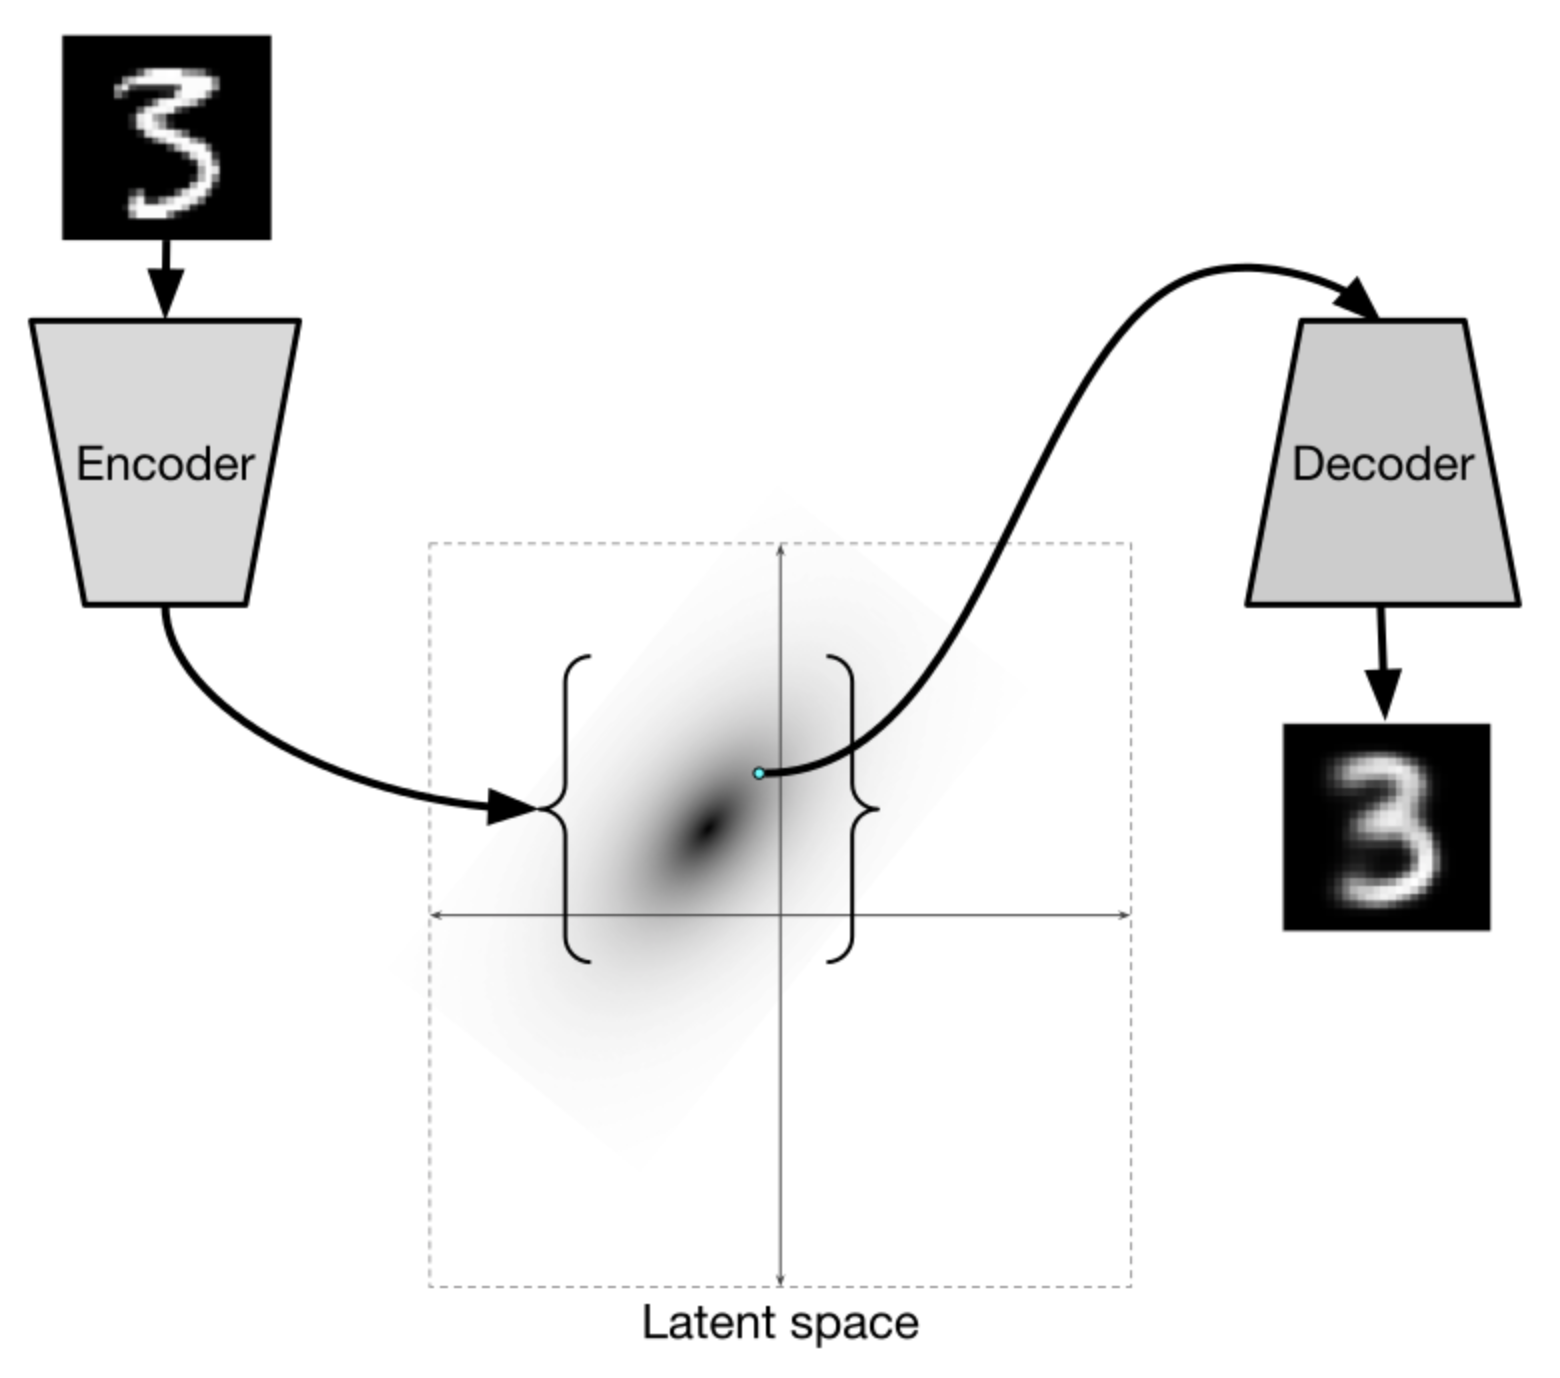
\includegraphics[width=\linewidth]{figs/VAE}
		\end{figure}
	\end{minipage}%
	\begin{minipage}[t]{0.4\columnwidth}
		\begin{figure}[h]
			\centering
			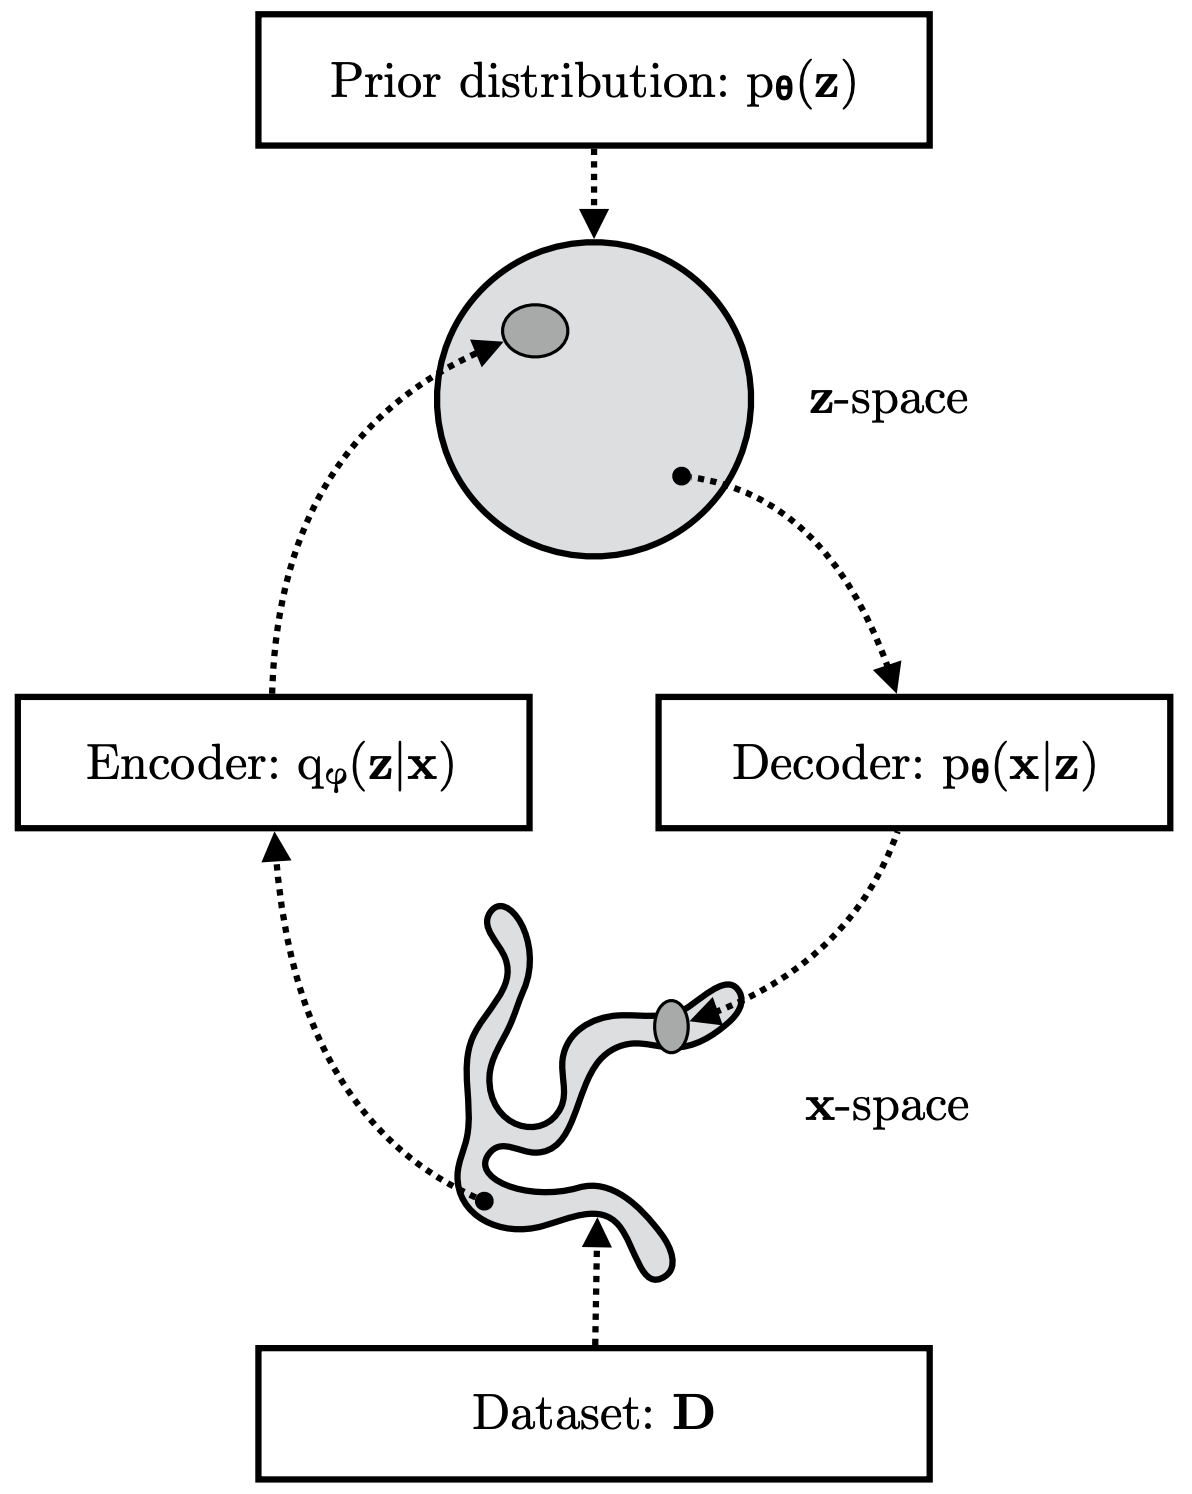
\includegraphics[width=\linewidth]{figs/vae_scheme}
		\end{figure}
	\end{minipage}
\end{frame}
%=======
\begin{frame}{Outline}
	\tableofcontents
\end{frame}
%=======
\section{Discrete VAE Latent Representations}
%=======
\begin{frame}{Discrete VAE Latents}
	\begin{block}{Motivation}
		\begin{itemize}
			\item Previous VAE models have used \textbf{continuous} latent variables $\bz$.
			\item For some modalities, \textbf{discrete} representations $\bz$ may be a more natural choice.
			\item Advanced autoregressive models (e.g., PixelCNN) are highly effective for distributions over discrete variables.
			\item Current transformer-like models process discrete tokens.
		\end{itemize}
	\end{block}
	\eqpause
	\begin{block}{ELBO}
		\vspace{-0.3cm}
		\[
			\cL_{\bphi, \btheta}(\bx)  = \bbE_{q_{\bphi}(\bz| \bx)} \log \pt(\bx| \bz) - \KL(q_{\bphi}(\bz| \bx) \| p(\bz)) \rightarrow \max_{\bphi, \btheta}.
		\]
		\vspace{-0.5cm}
	\end{block}
	\eqpause
	\begin{itemize}
		\item Apply the reparametrization trick to obtain unbiased gradients.
		\item Use Gaussian distributions for $q_{\bphi}(\bz| \bx)$ and $p(\bz)$ to compute the KL analytically.
	\end{itemize}
\end{frame}
%=======
\begin{frame}{Discrete VAE Latents}
	\begin{block}{Assumptions}
		\begin{itemize}
			\item Let $c \sim \Cat(\bpi)$, where 
			\vspace{-0.6cm}
			\[
			\bpi = (\pi_1, \dots, \pi_K), \quad \pi_k = P(c = k), \quad \sum_{k=1}^K \pi_k = 1.
			\]
			\vspace{-0.6cm}
			\item Suppose the VAE adopts a discrete latent variable $c$ with prior $p(c) = \text{Uniform}\{1, \dots, K\}$.
		\end{itemize}
	\end{block}
	\eqpause
	\begin{block}{ELBO}
		\vspace{-0.5cm}
		\[
			\cL_{\bphi, \btheta}(\bx)  = \bbE_{q_{\bphi}(c| \bx)} \log \pt(\bx| c) - {\color{olive} \KL(q_{\bphi}(c| \bx) \| p(c))} \rightarrow \max_{\bphi, \btheta}.
		\]
	\end{block}
	\vspace{-1.0cm}
	{\small
	\begin{multline*}
		{\color{olive} \KL(q_{\bphi}(c| \bx) \| p(c))} = \sum_{k=1}^K q_{\bphi}(k| \bx) \log \frac{q_{\bphi}(k| \bx)}{p(k)} 
		\nextonslide{= \\ = \color{violet}{\sum_{k=1}^K q_{\bphi}(k| \bx) \log q_{\bphi}(k| \bx)}  \color{teal}{- \sum_{k=1}^K q_{\bphi}(k| \bx) \log p(k)}}
		\nextonslide{= \\ = \color{violet}{- \Ent(q_{\bphi}(c| \bx))} + \color{teal}{\log K}. }
	\end{multline*}
	}
\end{frame}
%=======
\begin{frame}{Discrete VAE Latents}
	\myfootnotewithlink{https://arxiv.org/abs/2403.18103}{Chan S., Tutorial on Diffusion Models for Imaging and Vision, 2024}
	\[
		\cL_{\bphi, \btheta}(\bx)  = \bbE_{q_{\bphi}(c| \bx)} \log \pt(\bx| c) + \Ent(q_{\bphi}(c| \bx)) - \log K \rightarrow \max_{\bphi, \btheta}.
	\]
	\eqpause
	\vspace{-0.5cm}
	\begin{itemize}
		\item The encoder should output a discrete distribution $q_{\bphi}(c| \bx)$.
					\item We need an analogue of the reparametrization trick for discrete $q_{\bphi}(c| \bx)$.
		\item The decoder $\pt(\bx| c)$ must take a discrete random variable $c$ as input.
	\end{itemize}
	\begin{figure}[h]
		\centering
		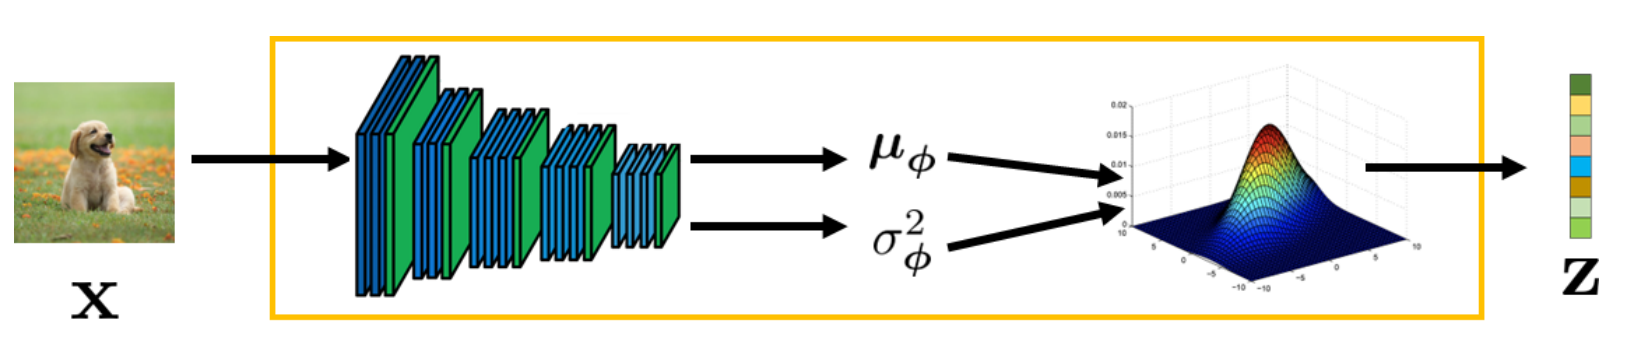
\includegraphics[width=0.7\linewidth]{figs/vae-encoder}
	\end{figure}
	\begin{figure}[h]
		\centering
		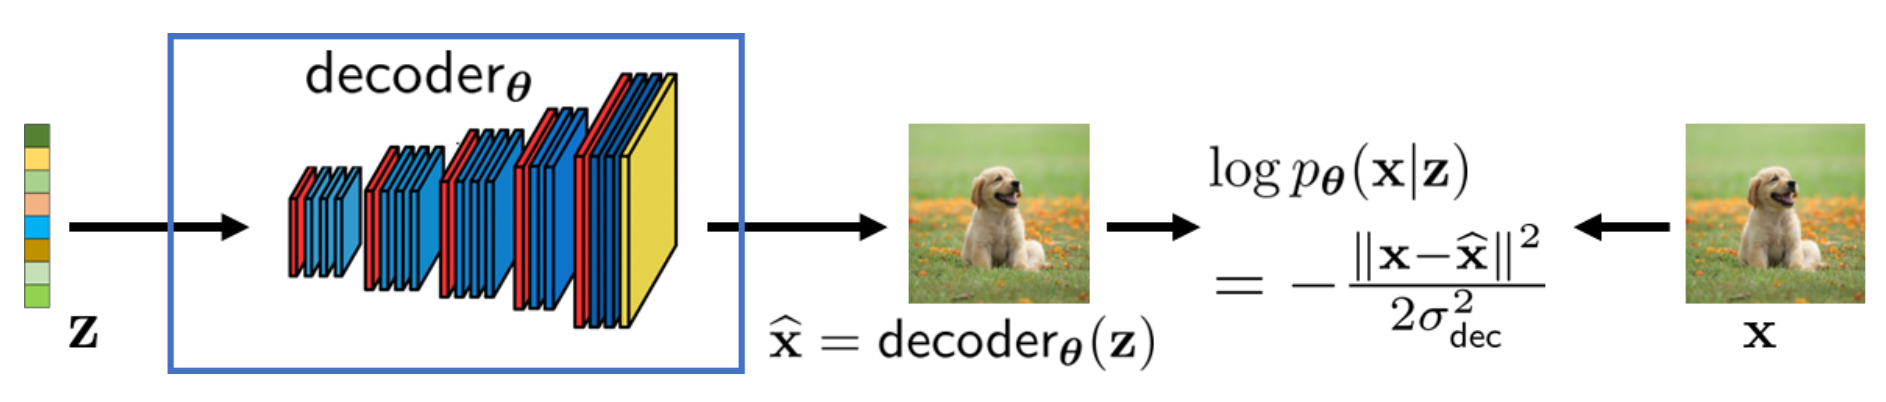
\includegraphics[width=0.9\linewidth]{figs/vae-decoder}
	\end{figure}
\end{frame}
%=======
\section{Vector Quantized VAE}
%=======
\begin{frame}{Vector Quantization}
	\myfootnotewithlink{https://arxiv.org/abs/2004.02088}{Zhao Y. et al. Feature Quantization Improves GAN Training, 2020} 
	Define the codebook (dictionary) space $\{\be_k\}_{k=1}^K$ with $\be_k \in \bbR^L$ and $K$ the number of codebook entries.
    \eqpause
	\begin{block}{Quantized Representation}
		A quantized vector $\bz_q \in \bbR^{L}$, for any $\bz \in \bbR^L$, is defined via nearest-neighbor lookup in the codebook:
		\vspace{-0.3cm}
		\[
			\bz_q = \bq (\bz) = \be_{k^*}, \quad \text{where } k^* = \argmin_k \| \bz - \be_k \|.
		\] 
		\vspace{-0.7cm}
	\end{block}
	\eqpause
	\vspace{-0.2cm}
	\begin{block}{Quantization Procedure}
		If the encoded tensor has spatial dimensions, quantization is independently applied to each of the $W \times H$ locations.
		\begin{minipage}[t]{0.65\columnwidth}
			\begin{figure}
				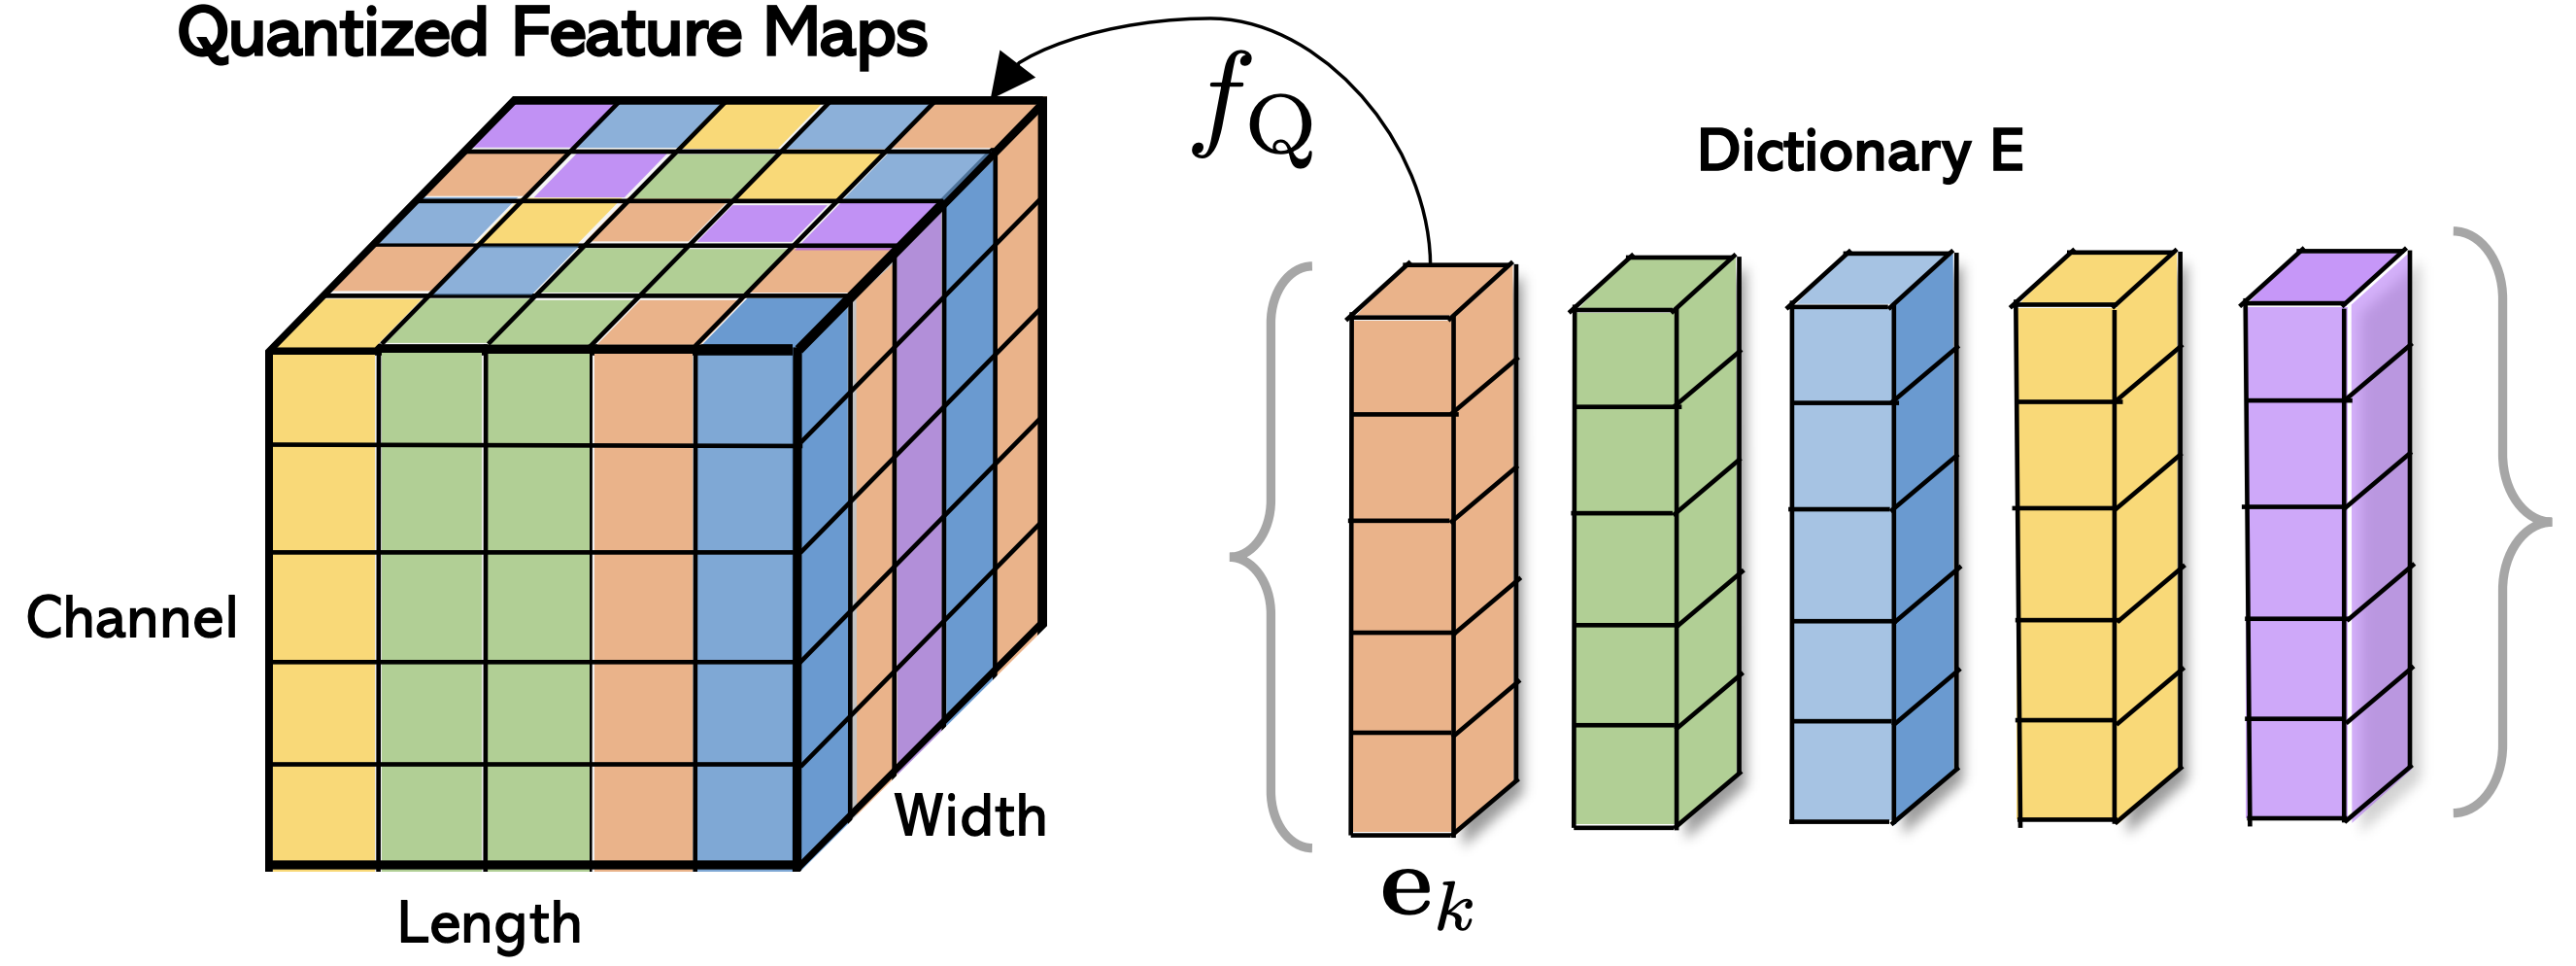
\includegraphics[width=0.8\linewidth]{figs/fqgan_cnn.png}
			\end{figure}
		\end{minipage}%
		\begin{minipage}[t]{0.35\columnwidth}
			\begin{figure}
				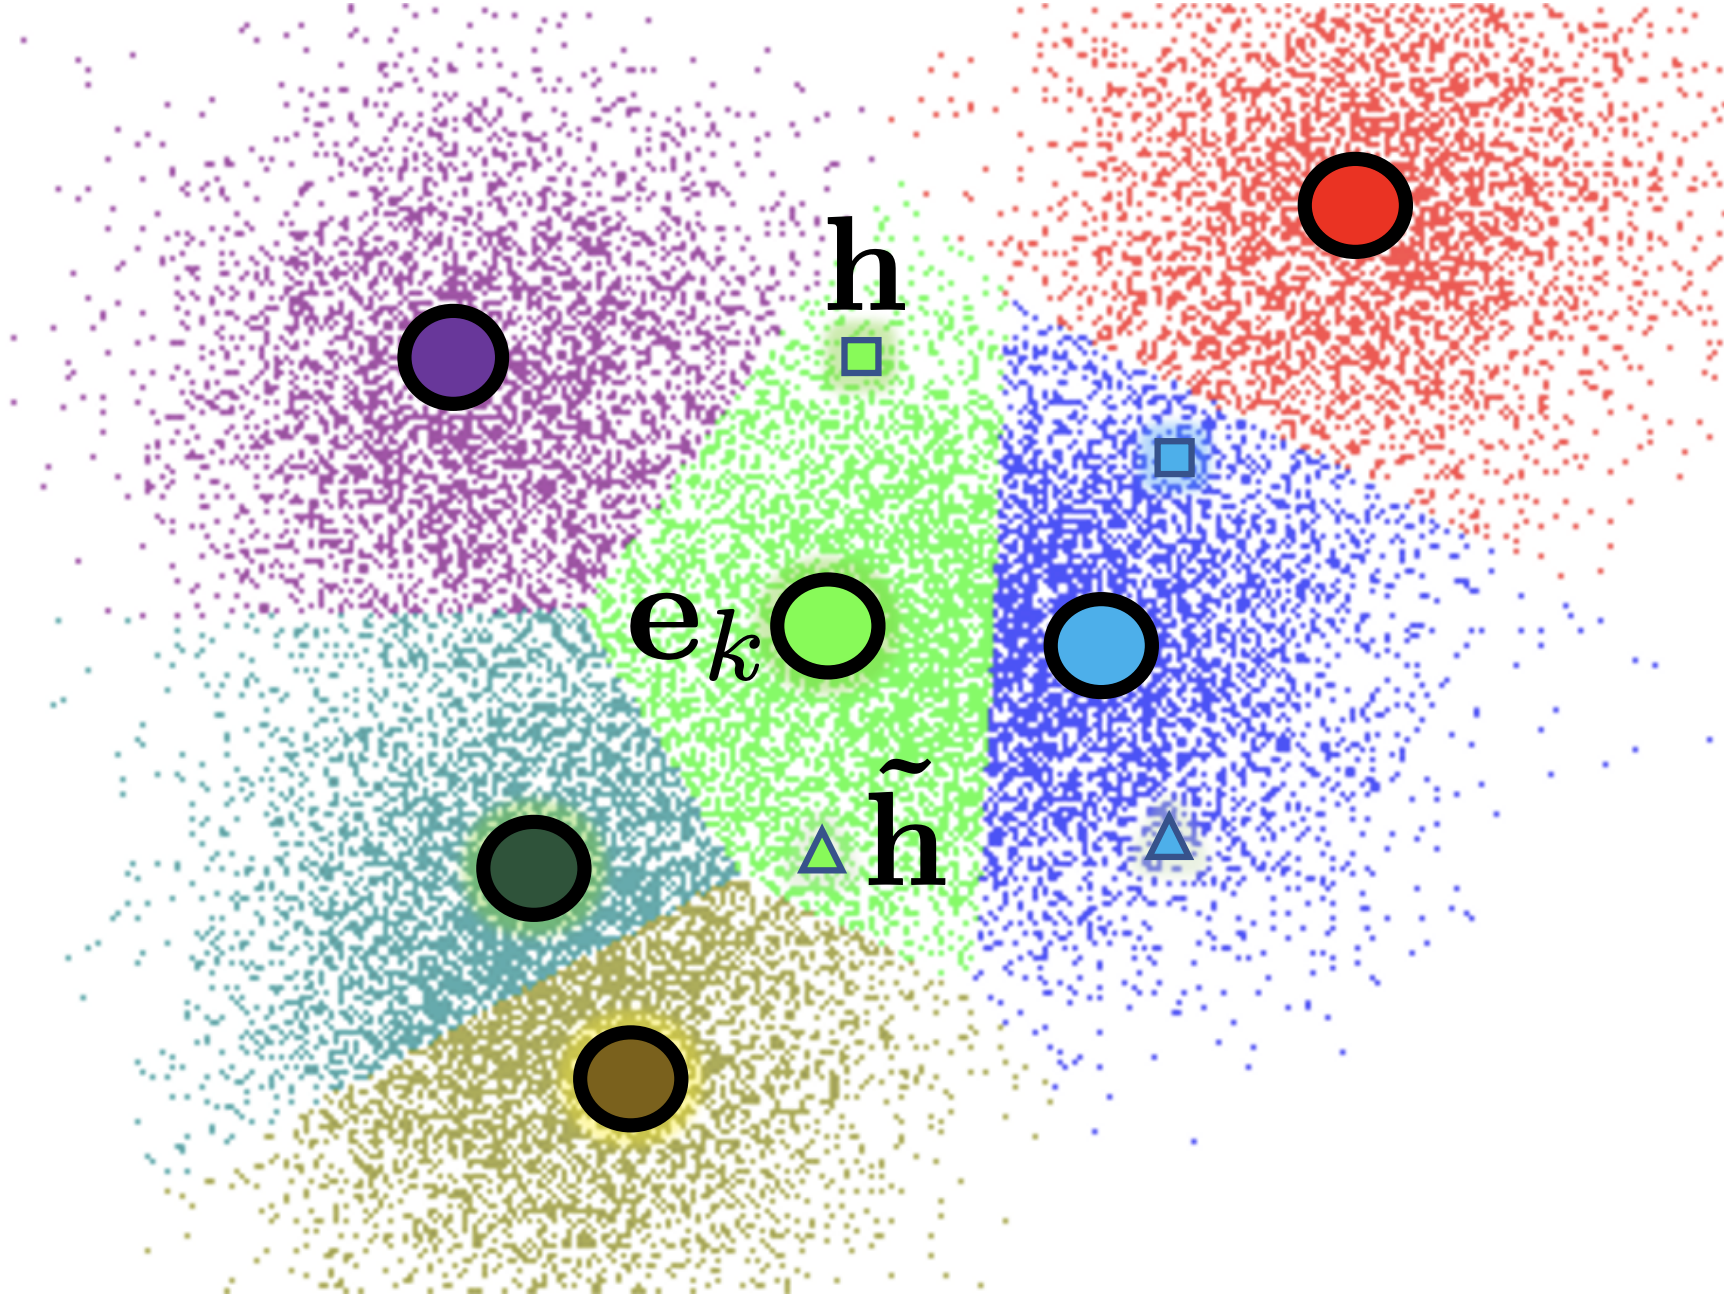
\includegraphics[width=0.7\linewidth]{figs/fqgan_lookup}
			\end{figure}
		\end{minipage}
	\end{block}
\end{frame}
%=======
\begin{frame}{Vector Quantized VAE (VQ-VAE)}
	\myfootnotewithlink{https://arxiv.org/abs/1711.00937}{Oord A., Vinyals O., Kavukcuoglu K. Neural Discrete Representation Learning, 2017} 
	\begin{itemize}
		\item The encoder outputs a continuous vector $\bz_e = \text{NN}_{e, \bphi}(\bx) \in \bbR^{L}$.
		\item Quantization deterministically maps $\bz_e$ to its quantized codebook vector $\bz_q$.
		\item The decoder is conditioned on codebook entries $\be_c$, i.e., via $\pt(\bx | \be_c)$ (instead of $\pt(\bx| c)$).
	\end{itemize}
    \eqpause
	\begin{block}{Deterministic Variational Posterior}
		\vspace{-0.3cm}
		\[
			q_{\bphi}(c = k^* | \bx) = \begin{cases}
				1 , \quad \text{for } k^* = \argmin_k \| \bz_e - \be_k \|; \\
				0, \quad \text{otherwise}.
		\end{cases}
		\]
        \eqpause
		\[
			\KL(q_{\bphi}(c| \bx) \| p(c)) = - \underbrace{\Ent(q_{\bphi}(c| \bx))}_{=0} + \log K = \log K. 
		\]
        \eqpause
	\end{block}	
	\vspace{-0.4cm}
	\textbf{Note:} The KL regularizer becomes constant and has no direct effect on the ELBO objective in this case.
\end{frame}
%=======
\begin{frame}{Vector Quantized VAE (VQ-VAE): Forward}
	\myfootnotewithlink{https://arxiv.org/abs/1711.00937}{Oord A., Vinyals O., Kavukcuoglu K. Neural Discrete Representation Learning, 2017} 
	\begin{block}{Deterministic Variational Posterior}
		\vspace{-0.3cm}
		\[
			q_{\bphi}(c = k^* | \bx) = \begin{cases}
			1 , \quad \text{if } k^* = \argmin_k \| \bz_e - \be_k \|; \\
			0, \quad \text{otherwise}.
			\end{cases}
		\]
	\vspace{-0.5cm}
	\end{block}	
    \eqpause
	\begin{block}{ELBO}
		\vspace{-0.6cm}
		\[
			\cL_{\bphi, \btheta}(\bx)  = \bbE_{q_{\bphi}(c| \bx)} \log \pt(\bx| \be_{c}) - \log K \nextonslide{= \log \pt(\bx| \bz_q) - \log K,}
		\]
		where $\bz_q = \be_{k^*}$, $k^* = \argmin_k \| \bz_e - \be_k \|$.
	\end{block}
    \eqpause
	\vspace{-0.3cm} 
	\begin{figure}
		\centering
		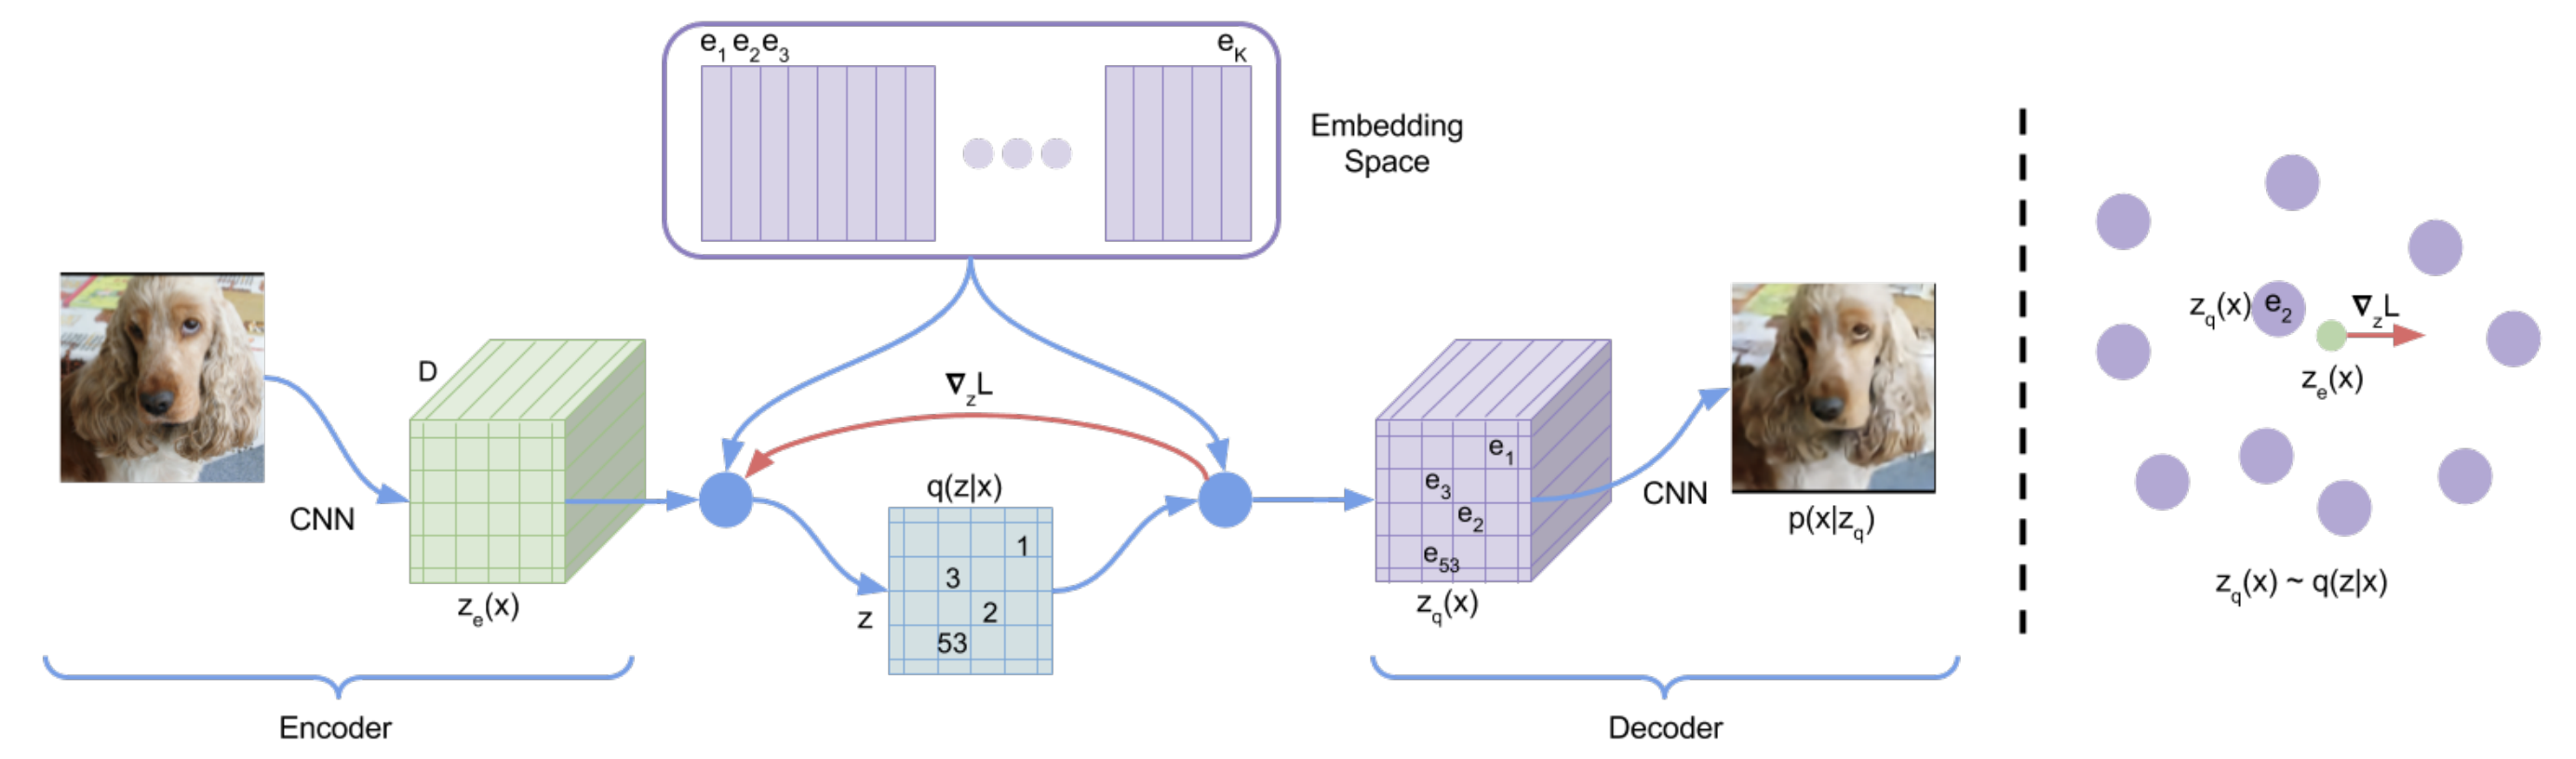
\includegraphics[width=0.85\linewidth]{figs/vqvae}
	\end{figure}
    \eqpause
	\vspace{-0.3cm} 
	\textbf{Challenge:} The $\argmin$ operation is non-differentiable.
\end{frame}
%=======
\begin{frame}{Vector Quantized VAE (VQ-VAE): Backward}
	\myfootnotewithlink{https://arxiv.org/abs/1711.00937}{Oord A., Vinyals O., Kavukcuoglu K. Neural Discrete Representation Learning, 2017} 
	\begin{block}{ELBO}
		\vspace{-0.5cm}
		\[
			\cL_{\bphi, \btheta}(\bx)  =  \log \pt(\bx| \bz_q) - \log K, \quad \bz_q = \be_{k^*},\; k^* = \argmin_k \| \bz_e - \be_k \|.
		\]
		\vspace{-0.5cm}
	\end{block}
    \eqpause
	\begin{figure}
		\centering
		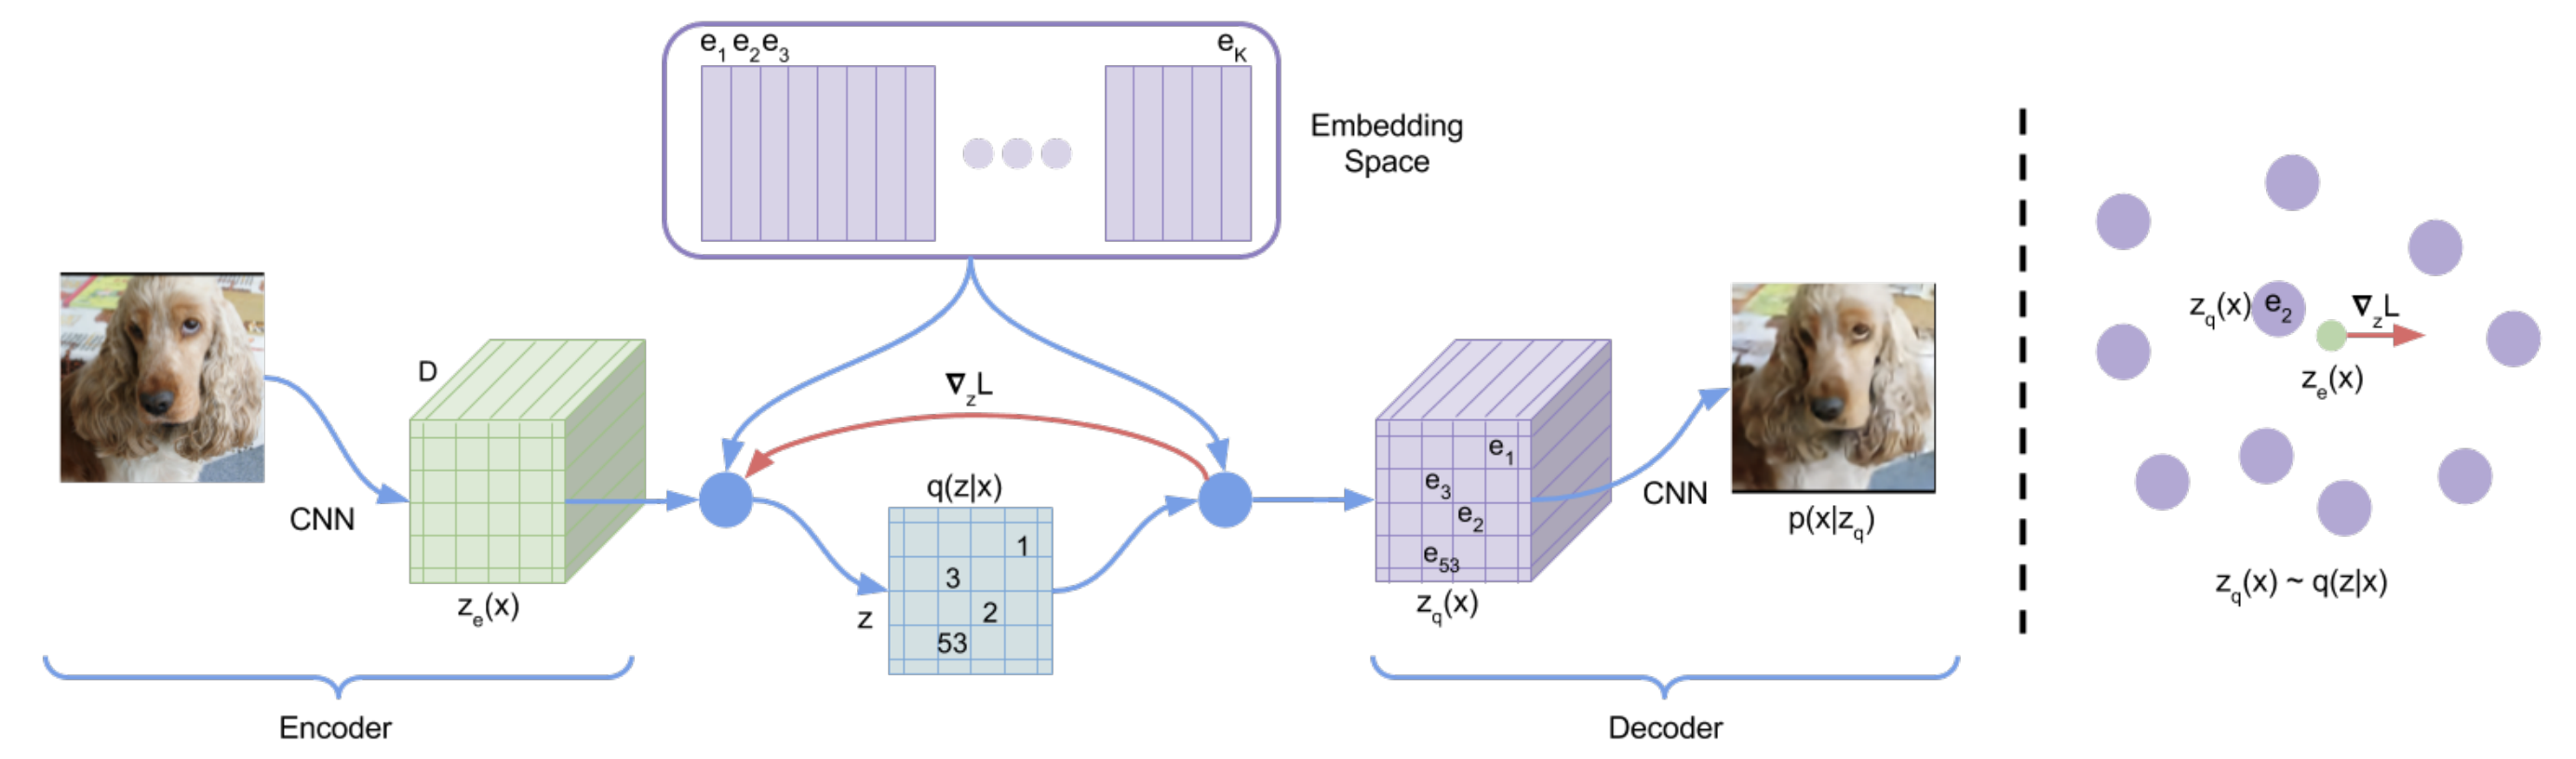
\includegraphics[width=0.85\linewidth]{figs/vqvae}
	\end{figure}
    \eqpause
	\vspace{-0.3cm}
	\begin{block}{Straight-Through Gradient Estimator}
		\vspace{-0.5cm}
		\begin{multline*}
		\frac{\partial \log p(\bx | \bz_q , \btheta)}{\partial \bphi} = \frac{\partial \log \pt(\bx| \bz_q)}{\partial \bz_q} \cdot {\color{red}\frac{\partial \bz_q}{\partial \bphi}} = \\
		\nextonslide{= \frac{\partial \log \pt(\bx| \bz_q)}{\partial \bz_q} \cdot {\color{red}\frac{\partial \bz_q}{\partial \bz_e}} \cdot \frac{\partial \bz_e}{\partial \bphi}}
		\nextonslide{\approx \frac{\partial \log \pt(\bx| \bz_q)}{\partial \bz_q} \cdot \frac{\partial \bz_e}{\partial \bphi}}
		\end{multline*}
	\end{block}
\end{frame}
%=======
\begin{frame}{Vector Quantized VAE-2 (VQ-VAE-2)}
	\myfootnotewithlink{https://arxiv.org/abs/1906.00446}{Razavi A., Oord A., Vinyals O. Generating Diverse High-Fidelity Images with VQ-VAE-2, 2019} 
	Extension to the spatial domain: $\bc \in \{1, \dots, K\}^{W \times H}$
	\vspace{-0.3cm}
	\[
		q_{\bphi}(\bc | \bx) = \prod_{i=1}^W \prod_{j=1}^H q(c_{ij} | \bx, \bphi); \quad p(\bc) = \prod_{i=1}^W \prod_{j=1}^H \text{Uniform}\{1, \dots, K\}.
	\]
	\vspace{-0.6cm}
	\begin{block}{Sample Diversity}
		\vspace{-0.2cm}
		\begin{figure}
			\centering
			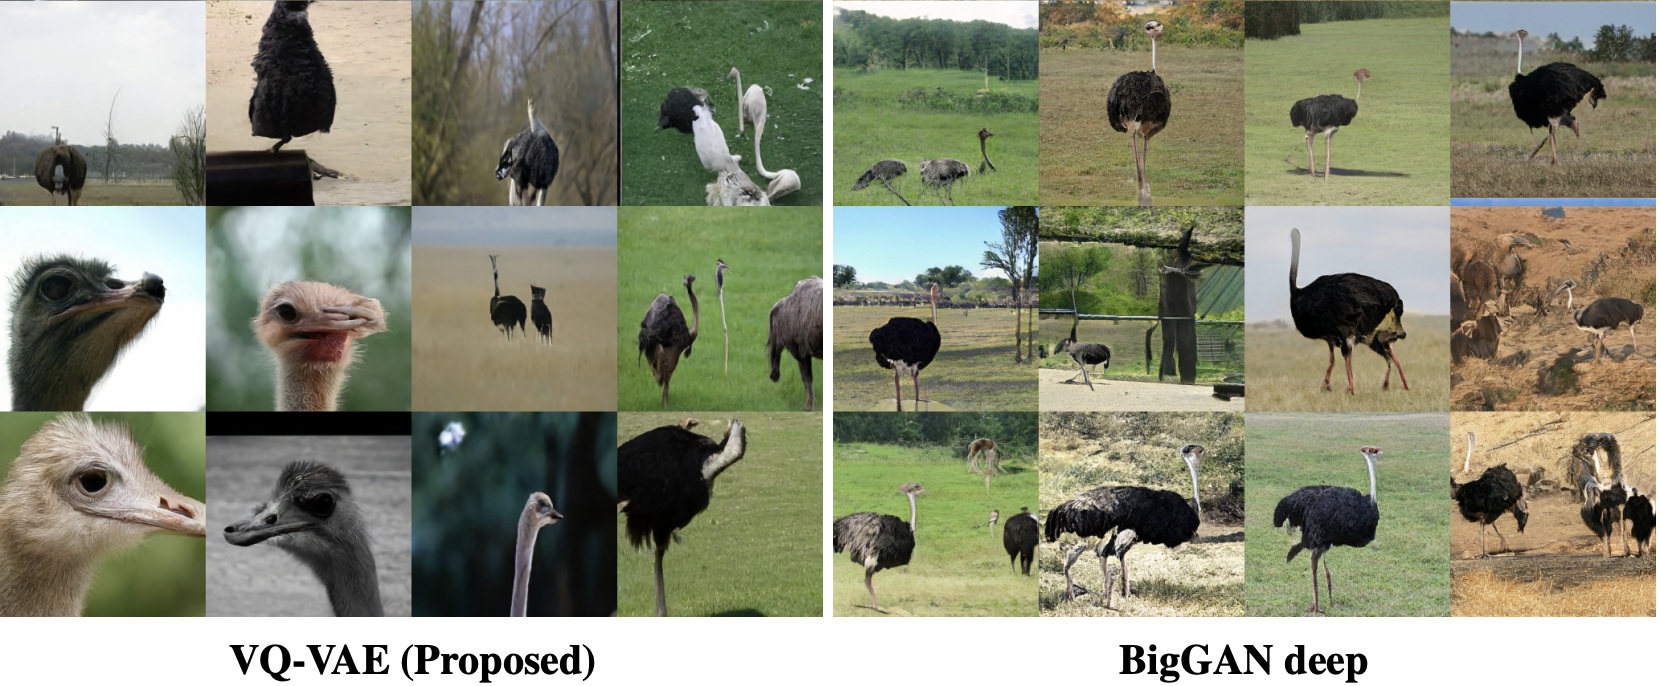
\includegraphics[width=1.0\linewidth]{figs/vqvae2_diversity}
		\end{figure}
	\end{block}
\end{frame}
%=======
\begin{frame}{Vector Quantized VAE (VQ-VAE): Final algorithm}
	\begin{block}{Training}
		\begin{itemize}
			\item Vector-quantize (per spatial location if applicable):
			\vspace{-0.3cm}
			\[
				k^* = \argmin_k \|\bz_e - \be_k\|_2, \quad \bz_q = \be_{k^*}, \quad \bz_e = \text{NN}_{e,\bphi}(\bx).
			\]
			\vspace{-0.5cm}
			\item Compute ELBO objective:
			\vspace{-0.3cm}
			\[
				\cL_{\bphi, \btheta}(\bx) = \log \pt(\bx | \bz_q) - \log K.
			\]
			\vspace{-0.5cm}
			\item Compute total loss with codebook and commitment losses (with stop-gradient $\text{sg}[\cdot]$):
			\vspace{-0.3cm}
			\[
				\cL = - \cL_{\bphi, \btheta}(\bx) + \big\|\text{sg}[\bz_e] - \be_{k^*}\big\|_2^2 + \beta \big\|\bz_e - \text{sg}[\be_{k^*}]\big\|_2^2
			\]
			\vspace{-0.5cm}
			\item Use straight-through gradient estimation for encoder.
		\end{itemize}
	\end{block}
	\eqpause
	\vspace{-0.3cm}
	\begin{block}{Sampling}
		\begin{itemize}
			\item Sample $c \sim p(c) = \text{Uniform}\{1, \dots, K\}$.
			\item Generate $\bx \sim \pt(\bx | \be_c)$.
		\end{itemize}
	\end{block}
\end{frame}
%=======
\section{ELBO Surgery}
%=======
\begin{frame}{ELBO Surgery}
	\myfootnotewithlink{http://approximateinference.org/accepted/HoffmanJohnson2016.pdf}{Hoffman M. D., Johnson M. J. ELBO Surgery: Yet Another Way to Carve Up the Variational Evidence Lower Bound, 2016}
	\vspace{-0.3cm}
	\[
	    \frac{1}{n} \sum_{i=1}^n \cL_{\bphi, \btheta}(\bx_i) = \frac{1}{n} \sum_{i=1}^n \Bigl[ \bbE_{q_{\bphi}(\bz| \bx_i)} \log \pt(\bx_i | \bz) - \KL(q_{\bphi}(\bz| \bx_i) \| p(\bz)) \Bigr].
	\]
    \eqpause
	\vspace{-0.3cm}
	\begin{block}{Theorem}
		\vspace{-0.5cm}
		\[
		    \frac{1}{n} \sum_{i=1}^n \KL(q_{\bphi}(\bz| \bx_i) \| p(\bz)) = {\color{violet} \KL(q_{\text{agg}, \bphi}(\bz) \| p(\bz))} + {\color{teal}\bbI_{q} [\bx, \bz]};
		\]
        \eqpause
		\vspace{-0.5cm}
		\begin{itemize}
			\item $q_{\text{agg}, \bphi}(\bz) = \frac{1}{n} \sum_{i=1}^n q_{\bphi}(\bz| \bx_i)$ denotes the \textbf{aggregated} variational posterior.
			\item $\bbI_{q} [\bx, \bz]$ is the mutual information between $\bx$ and $\bz$ under the data distribution $\pd(\bx)$ and $q_{\bphi}(\bz| \bx)$.
			\item  {\color{violet} The first term} encourages $q_{\text{agg}, \bphi}(\bz)$ to match the prior $p(\bz)$.
			\item {\color{teal} The second term} reduces the information about $\bx$ encoded in~$\bz$.
		\end{itemize}
	\end{block}
\end{frame}
%=======
\begin{frame}{ELBO Surgery}
	\myfootnotewithlink{http://approximateinference.org/accepted/HoffmanJohnson2016.pdf}{Hoffman M. D., Johnson M. J. ELBO Surgery: Yet Another Way to Carve Up the Variational Evidence Lower Bound, 2016}
		\vspace{-0.4cm}
		\[
		    \frac{1}{n} \sum_{i=1}^n \KL(q_{\bphi}(\bz| \bx_i) \| p(\bz)) = \KL(q_{\text{agg}, \bphi}(\bz) \| p(\bz)) + \bbI_q [\bx, \bz].
		\]
		\vspace{-0.3cm}
	\begin{block}{Proof}
		\vspace{-0.5cm}
		{\footnotesize
		\begin{multline*}
		    \frac{1}{n} \sum_{i=1}^n \KL(q_{\bphi}(\bz| \bx_i) \| p(\bz)) = \frac{1}{n} \sum_{i=1}^n \int q_{\bphi}(\bz| \bx_i) \log \frac{q_{\bphi}(\bz| \bx_i)}{p(\bz)} d \bz
		    \nextonslide{= \\= \frac{1}{n} \sum_{i=1}^n \int q_{\bphi}(\bz| \bx_i) \log \frac{{\color{violet}q_{\text{agg}, \bphi}(\bz)} {\color{teal}q_{\bphi}(\bz| \bx_i)}}{{\color{violet}p(\bz)} {\color{teal}q_{\text{agg}, \bphi}(\bz)}} d \bz}
		    \nextonslide{= \\ = \int \frac{1}{n} \sum_{i=1}^n  q_{\bphi}(\bz| \bx_i) \log {\color{violet}\frac{q_{\text{agg}, \bphi}(\bz)}{p(\bz)}} d \bz + \frac{1}{n}\sum_{i=1}^n \int q_{\bphi}(\bz| \bx_i) \log {\color{teal}\frac{q_{\bphi}(\bz| \bx_i)}{q_{\text{agg}, \bphi}(\bz)}} d \bz}
		    \nextonslide{= \\ = \KL (q_{\text{agg}, \bphi}(\bz) \| p(\bz)) + \frac{1}{n}\sum_{i=1}^n \KL(q_{\bphi}(\bz| \bx_i) \| q_{\text{agg}, \bphi}(\bz))}
		\end{multline*}
        \eqpause
		}
		\vspace{-0.4cm}
		\[
			\bbI_{q} [\bx, \bz] = \frac{1}{n}\sum_{i=1}^n \KL(q_{\bphi}(\bz| \bx_i) \| q_{\text{agg}, \bphi}(\bz)).
		\]
	\end{block}
\end{frame}
%=======
\begin{frame}{ELBO Surgery}
	\myfootnotewithlink{http://approximateinference.org/accepted/HoffmanJohnson2016.pdf}{Hoffman M. D., Johnson M. J. ELBO Surgery: Yet Another Way to Carve Up the Variational Evidence Lower Bound, 2016}
	\vspace{-0.3cm}
	\begin{block}{Revisiting the ELBO}
		\vspace{-0.7cm}
		{\small
		\begin{multline*}
		    \frac{1}{n}\sum_{i=1}^n \cL_{\bphi, \btheta}(\bx_i) = \frac{1}{n} \sum_{i=1}^n \left[ \bbE_{q_{\bphi}(\bz| \bx_i)} \log \pt(\bx_i | \bz) - \KL(q_{\bphi}(\bz| \bx_i) \| p(\bz)) \right]
		    \nextonslide{= \\ = \underbrace{\frac{1}{n} \sum_{i=1}^n \bbE_{q_{\bphi}(\bz| \bx_i)} \log \pt(\bx_i | \bz)}_{\text{Reconstruction Loss}} - \underbrace{\vphantom{ \sum_{i=1}^n} \bbI_q [\bx, \bz]}_{\text{Mutual Information}} - \underbrace{\vphantom{ \sum_{i=1}^n} \KL(q_{\text{agg}, \bphi}(\bz) \| {\color{teal}p(\bz)})}_{\text{Marginal KL}}}
		\end{multline*}
		}
		\vspace{-0.3cm}
	\end{block}
    \eqpause
	The prior distribution $p(\bz)$ only appears in the last term.
    \eqpause
	\begin{block}{Optimal VAE Prior}
		\vspace{-0.7cm}
		\[
	  		\KL(q_{\text{agg}, \bphi}(\bz) \| p(\bz)) = 0 \quad \Leftrightarrow \quad p (\bz) = q_{\text{agg}, \bphi}(\bz) = \frac{1}{n} \sum_{i=1}^n q_{\bphi}(\bz| \bx_i).
		\]
        \eqpause
		\vspace{-0.4cm} \\
		Hence, the optimal prior $p(\bz)$ is the aggregated variational posterior $q_{\text{agg}, \bphi}(\bz)$.
	\end{block}
\end{frame}
%=======
\begin{frame}{Marginal KL}
	\myfootnotewithlink{https://arxiv.org/abs/1505.05770}{Rezende D. J., Mohamed S. Variational Inference with Normalizing Flows, 2015} 
	\[
		\KL(q_{\text{agg}, \bphi}(\bz) \| p(\bz))
	\]
	\vspace{-0.5cm}
	\begin{itemize}
		\item $q_{\bphi}(\bz| \bx) = \cN(\bmu_{\bphi}(\bx), \bsigma^2_{\bphi}(\bx))$ is unimodal. 
		\item It is generally believed that the \textbf{mismatch between} $p(\bz)$  \textbf{and} $q_{\text{agg}, \bphi}(\bz)$  is the primary explanation for blurry VAE-generated images.
	\end{itemize}
    \eqpause
	\begin{figure}
		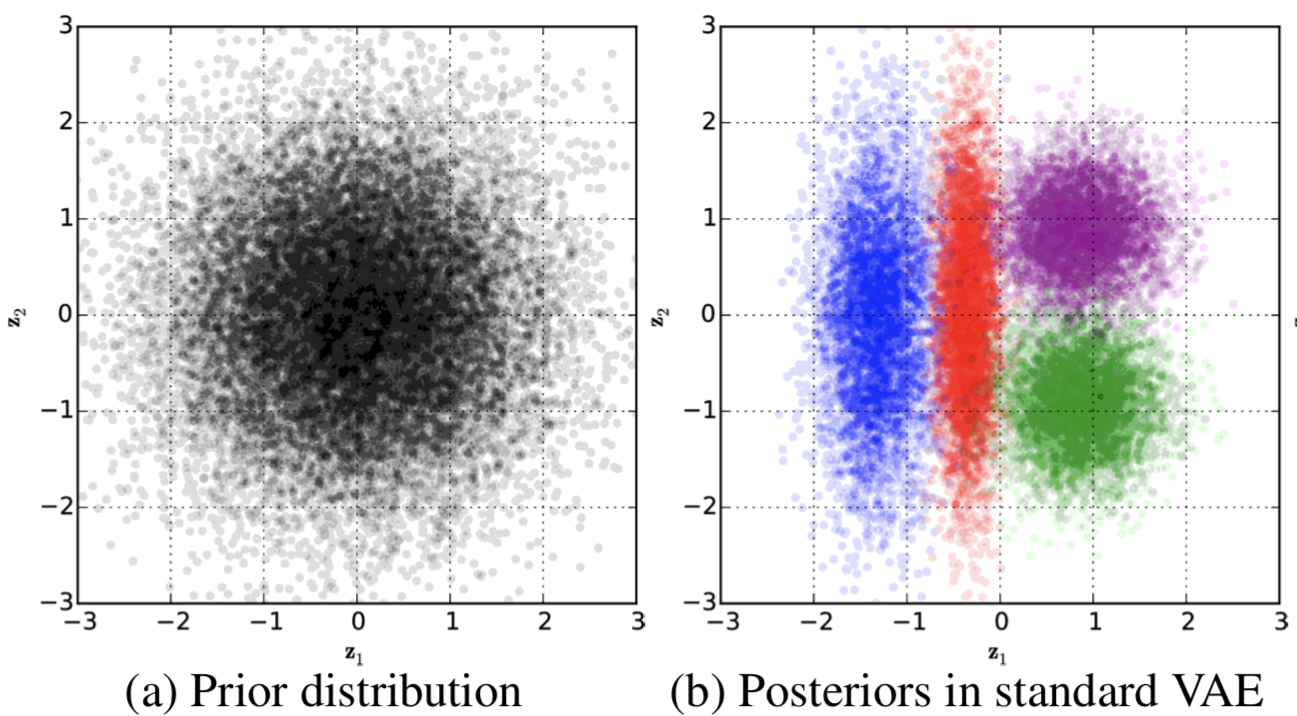
\includegraphics[width=0.8\linewidth]{figs/agg_posterior}
	\end{figure}
\end{frame}
%=======
\section{Learnable VAE Prior}
%=======
\begin{frame}{Optimal VAE Prior}
	\myfootnotewithlink{https://jmtomczak.github.io/blog/7/7\_priors.html}{image credit: https://jmtomczak.github.io/blog/7/7\_priors.html}
	\begin{itemize}
		\item Standard Gaussian $p(\bz) = \cN(0, \bI)$ often leads to over-regularization.
		\item $p(\bz) = q_{\text{agg}, \bphi}(\bz) = \frac{1}{n}\sum_{i=1}^n q_{\bphi}(\bz| \bx_i)$ risks overfitting and incurs high computational cost.
	\end{itemize}
    \eqpause
	\vspace{-0.5cm}
	\begin{minipage}[t]{0.5\columnwidth}
		\begin{block}{Non-Learnable Prior $p(\bz)$}
			\begin{figure}[h]
				\centering
				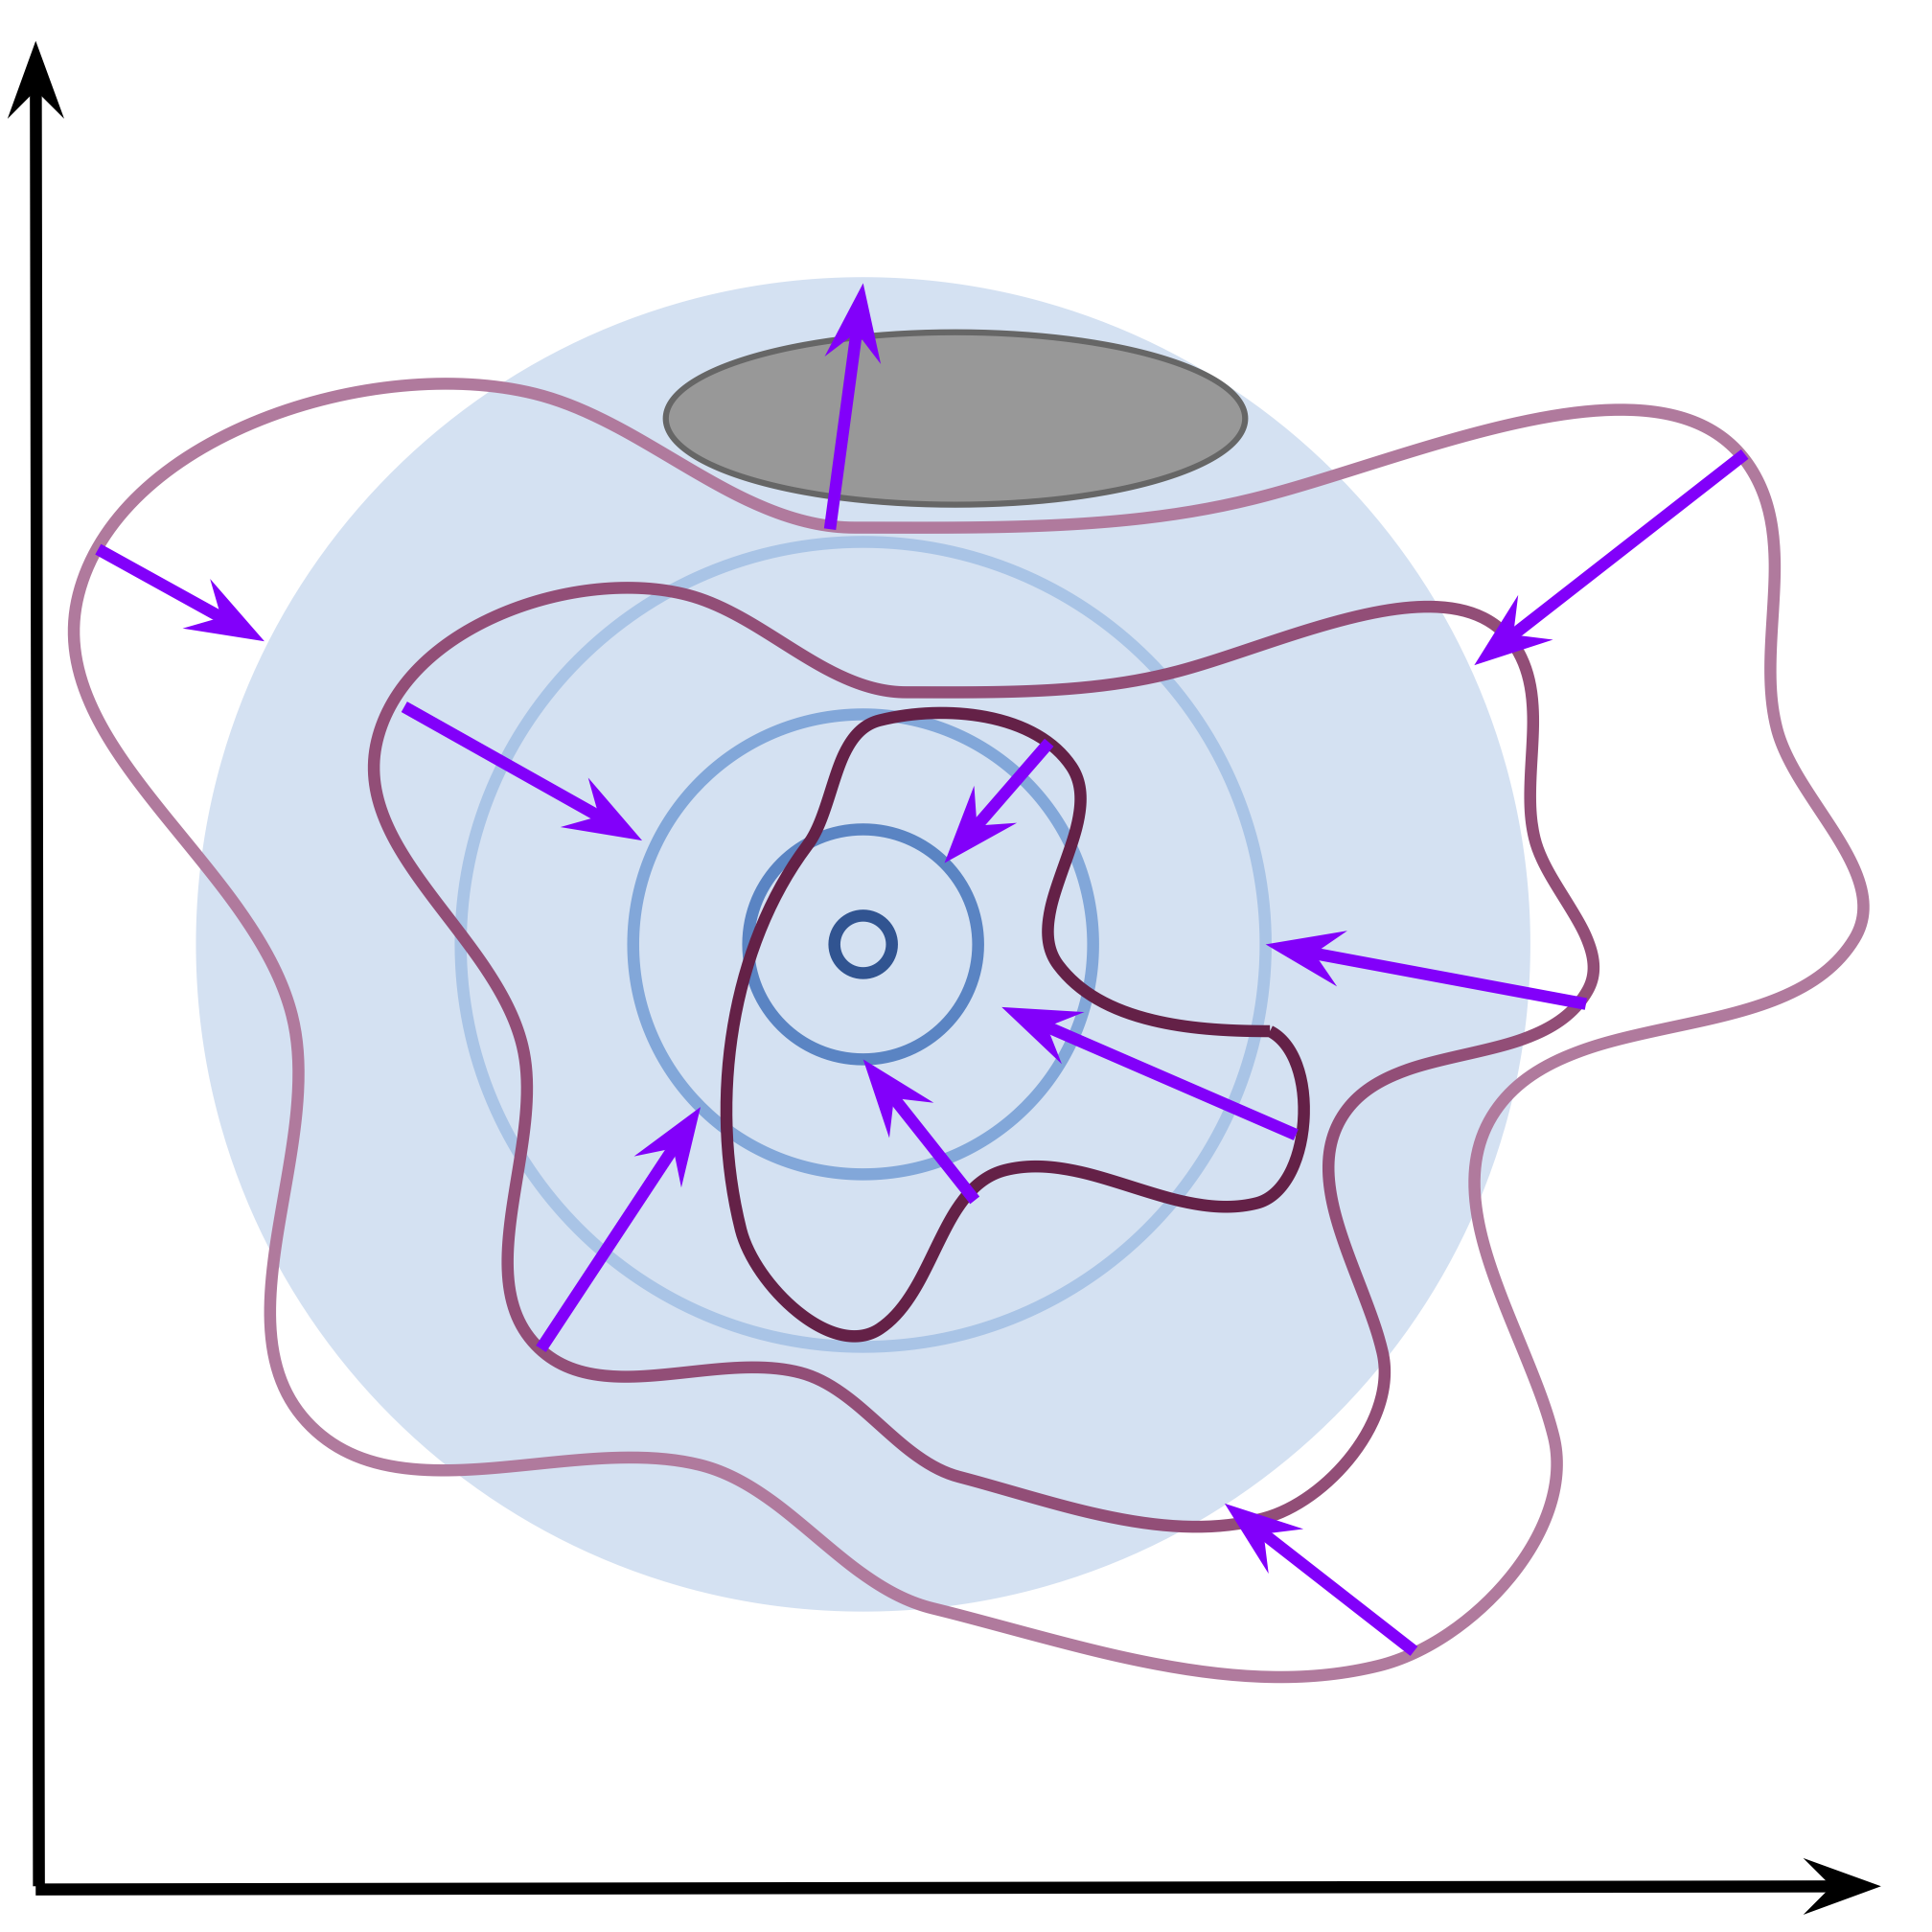
\includegraphics[width=0.6\linewidth]{figs/non_learnable_prior}
			\end{figure}
		\end{block}
	\end{minipage}%
	\begin{minipage}[t]{0.5\columnwidth}
		\begin{block}{Learnable Prior $p_{\blambda}(\bz)$}
			\begin{figure}[h]
				\centering
				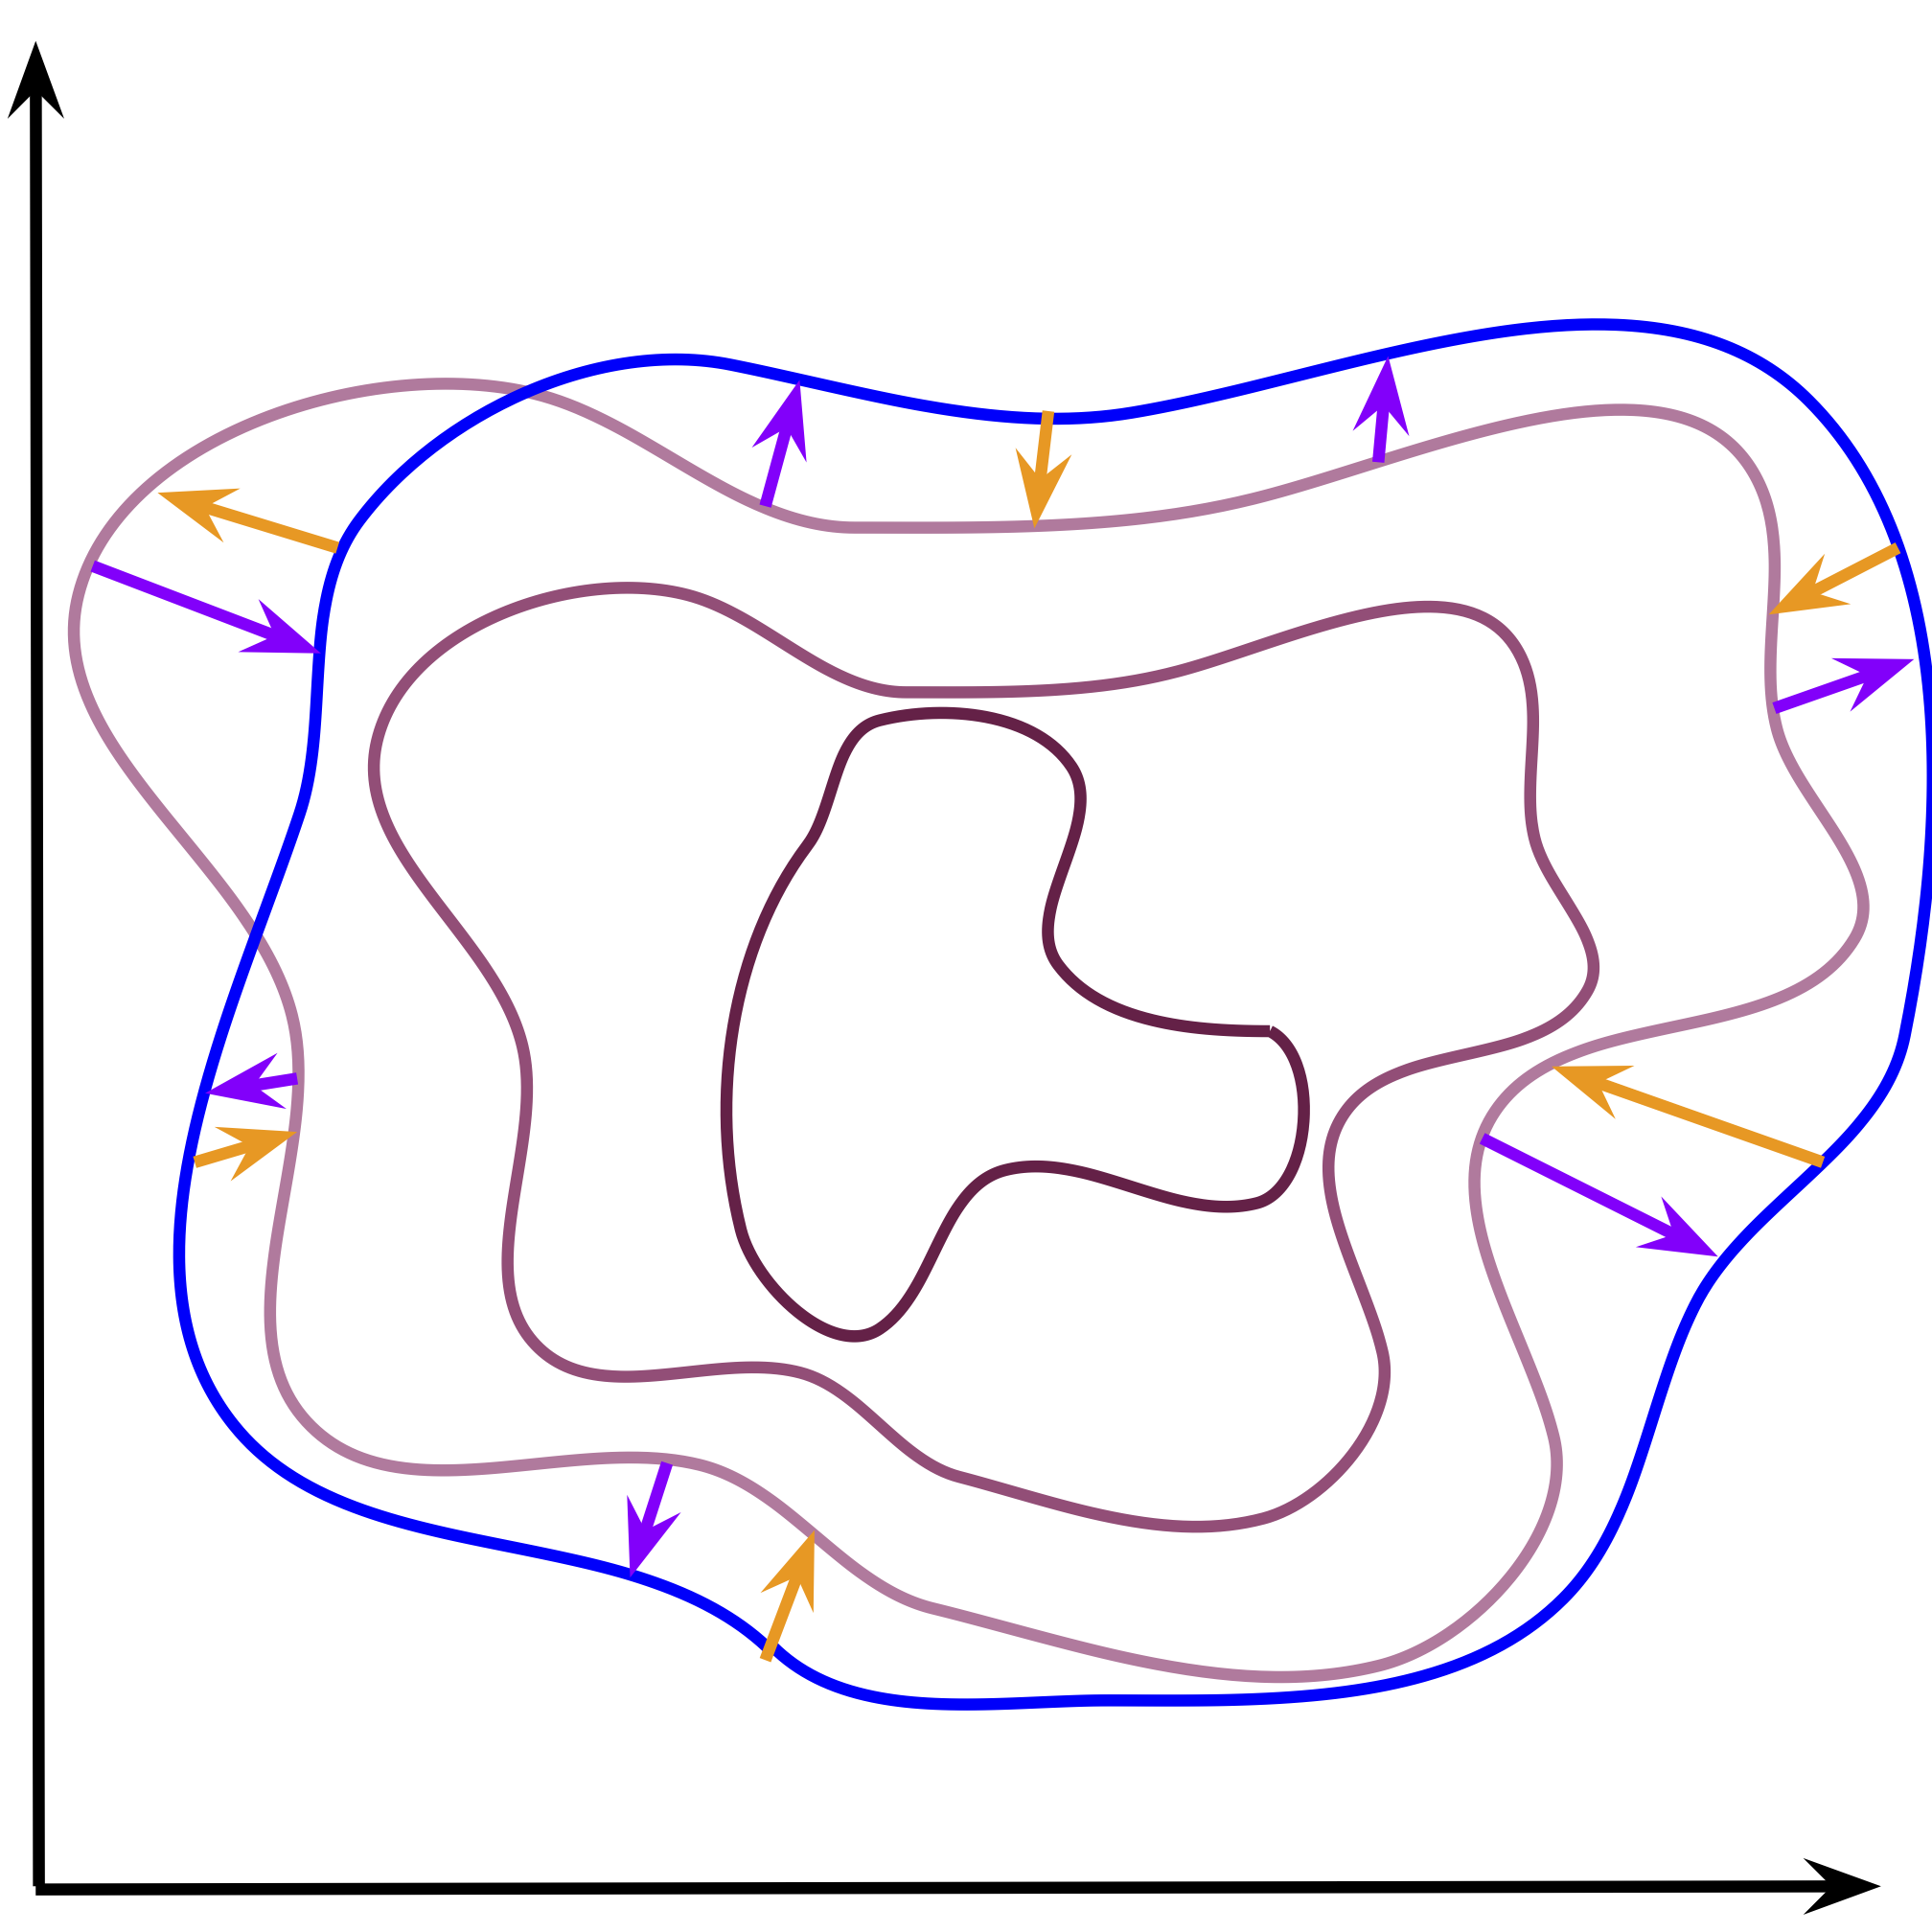
\includegraphics[width=0.6\linewidth]{figs/learnable_prior}
			\end{figure}
		\end{block}
	\end{minipage}
    \eqpause
	\vspace{-0.3cm}
	\[
	\frac{1}{n}\sum_{i=1}^n \cL_{\bphi, \btheta}(\bx_i) = \text{RL} - \text{MI} -  \KL(q_{\text{agg}, \bphi}(\bz) \| {\color{teal}p_{\blambda}(\bz)})
	\]
	This is the forward KL divergence with respect to $p_{\blambda}(\bz)$.
\end{frame}
%=======
\begin{frame}{NF-Based VAE Prior}
	\myfootnotewithlink{https://arxiv.org/abs/1611.02731}{Chen X. et al. Variational Lossy Autoencoder, 2016}
	\begin{block}{NF Model in Latent Space}
		\vspace{-0.5cm}
		\[
			\log p_{\blambda}(\bz) = \log p(\bz^*) + \log  \left | \det \left(\frac{d \bz^*}{d\bz}\right)\right| = \log p(\bff_{\blambda}(\bz)) + \log \left | \det (\bJ_\bff)\right| 
		\]
		\vspace{-0.3cm}
		\[
			\bz = \bg_{\blambda}(\bz^*) = \bff^{-1}_{\blambda}(\bz^*)
		\]
	\end{block}
    \eqpause
	\vspace{-0.3cm}
	\begin{itemize}
		\item RealNVP with coupling layers,
		\item Autoregressive normalizing flows (efficient $\bff_{\blambda}(\bz)$, but $\bg_{\blambda}(\bz^*)$ can be slow).
	\end{itemize}
    \eqpause
	\begin{block}{ELBO with NF-Based VAE Prior}
		\vspace{-0.5cm}
		{\small
			\begin{multline*}
				\cL_{\bphi, \btheta}(\bx) = \bbE_{q_{\bphi}(\bz| \bx)} \log \pt(\bx| \bz) - \KL(q_{\bphi}(\bz| \bx) \| p(\bz))
				\nextonslide{= \\ = \bbE_{q_{\bphi}(\bz| \bx)} \left[ \log \pt(\bx | \bz) + {\color{violet}\log p_{\blambda}(\bz)} - \log q_{\bphi}(\bz| \bx) \right]}
				\nextonslide{= \\ = \bbE_{q_{\bphi}(\bz| \bx)} \Bigl[ \log \pt(\bx | \bz) + \underbrace{ \Bigl({\color{violet} \log p(\bff_{\blambda}(\bz)) + \log \left| \det (\bJ_\bff) \right|} \Bigr) }_{\text{NF-based prior}} - \log q_{\bphi}(\bz| \bx) \Bigr]} 
			\end{multline*}
		}
	\end{block}
\end{frame}
%=======
\begin{frame}{Summary}
	\begin{itemize}
		\item Discrete VAE latents offer a natural class of latent variable models.	
		\vfill
		\item Vector quantization provides a way to construct VAEs with discrete latents and deterministic variational posteriors.
		\vfill
		\item The straight-through gradient estimator allows gradients to pass as if quantization were an identity operation during backpropagation.			
		\vfill
		\item ELBO surgery gives insights into the prior's influence in VAEs; the optimal prior is the aggregated variational posterior. 
		\vfill
		\item The mismatch between $p(\bz)$ and $q_{\text{agg}, \bphi}(\bz)$ is widely regarded as the principal reason for VAE-generated image blurriness.
		\vfill
		\item Normalizing flow-based priors, including autoregressive flows, can be incorporated directly into VAEs.	
	\end{itemize}
\end{frame}
%=======
\end{document}